\documentclass[]{scrartcl}

% Load packages to allow in- and output of non-ASCII characters.
\usepackage{lmodern}        % Use an extension of the original Computer Modern font to minimize the use of bitmapped letters.
\usepackage[T1]{fontenc}    % Determines font encoding of the output. Font packages have to be included before this line.
\usepackage[utf8]{inputenc} % Determines encoding of the input. All input files have to use UTF8 encoding.

% Extended LaTeX functionality is enables by including packages with \usepackage{...}.
\usepackage{fixltx2e}   % Provides fixes for several errors in LaTeX2e.
\usepackage{amsmath}    % Extended typesetting of mathematical expression.
\usepackage{amssymb}    % Provides a multitude of mathematical symbols.
\usepackage{mathtools}  % Further extensions of mathematical typesetting.
\usepackage{microtype}  % Small-scale typographic enhancements.
\usepackage{enumitem}   % User control over the layout of lists (itemize, enumerate, description).
\usepackage{multirow}   % Allows table elements to span several rows.
\usepackage{booktabs}   % Improves the typesettings of tables.
\usepackage{subcaption} % Allows the use of subfigures and enables their referencing.
\usepackage[ruled,linesnumbered,algochapter]{algorithm2e} % Enables the writing of pseudo code.
\usepackage[usenames,dvipsnames,table]{xcolor} % Allows the definition and use of colors. This package has to be included before tikz.
\usepackage{nag}       % Issues warnings when best practices in writing LaTeX documents are violated.
\usepackage{hyperref}  % Enables cross linking in the electronic document version. This package has to be included second to last.
%-- \usepackage[acronym,toc]{glossaries} % Enables the generation of  glossaries and lists fo acronyms. This package has to be included last.


\usepackage{graphicx}
% Packages
\usepackage{soul}
\usepackage{caption}
\usepackage{amsthm}
\usepackage{listings}
\usepackage{subcaption}
\usepackage[utf8]{inputenc}
\usepackage{framed}
\usepackage{booktabs}
% \usepackage[colorlinks=true, linkcolor=DeepBlue, citecolor=DeepGreen]{hyperref}
\usepackage{mathtools}
\usepackage{todonotes}
\usepackage{realboxes}


% Tikz
\usepackage{tikz}
\usetikzlibrary{calc}
\usetikzlibrary{arrows.meta}
\usetikzlibrary{intersections}
\usetikzlibrary{positioning}
\usetikzlibrary{shapes}
\usetikzlibrary{arrows}
\usetikzlibrary{fit}

\usepackage{pgfplots}

\setlist{topsep=1mm}

% Theorems
\makeatletter
\newtheoremstyle{break}
   {\topsep}{\topsep}%
   {\itshape}{}%
   {\bfseries}{}%
   { }
   {\thmname{#1}\thmnumber{\@ifnotempty{#1}{ }\@upn{#2}}%
    \thmnote{ {\bfseries(#3)}}.}% 
\makeatother
\theoremstyle{break}

\newtheorem{thm}{Theorem}
\newtheorem{definition}[thm]{Definition}
\newtheorem{invariant}[thm]{Invariant}
\newtheorem{example}[thm]{Example}
\newtheorem{notation}[thm]{Notation}

% Basic fluff
\newcommand{\ellipses}{\textnormal{[\,\dots]}\ }
\newcommand{\mt}[1]{\textnormal{#1}}
\renewcommand{\tt}[1]{\texttt{#1}}
\colorlet{shadecolor}{yellow!60}
\newcommand{\highlight}[1]{\colorbox{yellow!70}{#1}}
\newcommand{\shade}[1]{\begin{shaded}#1\end{shaded}}
\newcommand{\tuple}[1]{\ensuremath{\langle #1 \rangle}}
\newcommand{\lp}{{\textnormal (}}
\newcommand{\rp}{{\textnormal )}}
\newcommand{\paren}[1]{\lp{#1}\rp}
% Graph Cartesian product
\newcommand{\gcp}{\Box}
\newcommand{\floor}[1]{\left\lfloor{#1}\right\rfloor}
\newcommand{\ceil}[1]{\left\lceil{#1}\right\rceil}
\newcommand{\degs}{{^\circ}}

% Blackboard bold letters, quantors
\newcommand{\N}{\mathbb{N}}
\newcommand{\Q}{\mathbb{Q}}
\newcommand{\R}{\mathbb{R}}
\newcommand{\B}{\mathbb{B}}
\newcommand{\C}{\mathbb{C}}
\newcommand{\allQ}[1]{\left[\forall #1 \right]}
\newcommand{\muQ}[1]{\left[\mu #1 \right]}
\newcommand{\exQ}[1]{\left[\exists #1 \right]}

% Symbol for the extended Wumpus world.
\newcommand{\wext}{\ensuremath{\mathcal{W}_{\mathrm{ext}}}}
\newcommand{\wjun}{\ensuremath{\mathcal{W}_{\mathrm{jun}}}}
\newcommand{\ssem}{\ensuremath{\mathrm{sem}}}

\newcommand{\dist}[2]{||{#1},{#2}||}
\newcommand{\dlvhex}{DLVhex}
\newcommand{\acthex}{\textsc{acthex}}
\newcommand{\aspR}{\coloneq}

% Logic programs
\newcommand{\aspHead}[1]{\ensuremath{\mathrm{head}(#1)}}
\newcommand{\aspBodyP}[1]{\ensuremath{\mathrm{body}^+(#1)}}
\newcommand{\aspBodyM}[1]{\ensuremath{\mathrm{body}^-(#1)}}
\newcommand{\aspRule}[2]{\ensuremath{#1 \leftarrow #2}}

% personalities
\newcommand{\personality}[5]{\tuple{\type{#1},\type{#2}, \type{#3}, \type{#4}, \type{#5}}}

\newenvironment{emquote}{\begin{quote}\em}{\end{quote}}


\newcommand{\stdlisting}{%
    \lstset{
        basicstyle=\ttfamily,
        frame=single,
        captionpos=b,
        rulecolor=\color{gray},
        backgroundcolor=\color{VeryLightGray},
        tabsize=4,
        showtabs=false,
        float=t,
        showspaces=false,
        showstringspaces=false,
        framexleftmargin=0.3cm,
        xleftmargin=0.3cm,
        framextopmargin=0.2cm,
        framexbottommargin=0.2cm,
    }%
}
\newcommand{\co}{\mathbf{Co}}
\newcommand{\cansend}[2]{#1 \rightarrowtail \{#2\}}
\newcommand{\cantsend}[2]{#1 \multimap \{#2\}}
\newcommand{\canrec}[2]{\{#1\} \rightarrowtail #2}
\newcommand{\cantrec}[2]{\{#1\} \multimap #2}
\newcommand{\rec}[1]{\field{rec}(#1)}
\newcommand{\ft}[1]{\tt{ft}_{#1}}
\renewcommand{\int}[1]{\tt{int}_{#1}}
\newcommand{\proc}[1]{\tt{proc}_{#1}}
\newcommand{\sends}[3]{#1 \rightarrow [#2] \rightarrow #3}
\newcommand{\sendsm}[4]{#1 \rightarrow [#2 , #3] \rightarrow #4}
\newcommand{\sendsf}[6]{#1\langle #2 \rangle \rightarrow [#3,#4] \rightarrow \langle#5\rangle#6}

\newcommand{\compT}[2]{\tt{Comp}_{#1,#2}}

\newcommand{\field}[1]{\mathtt{#1}}

\newcommand{\verbatimTT}[1]{\texttt{#1}}

\DeclareMathOperator{\tint}{int}
\newcommand{\type}[1]{\mathtt{#1}}
\DeclareMathOperator{\cint}{cint}

\newcommand{\action}[1]{\ensuremath{\mathsf{#1}}}
\definecolor{PaleRed}{RGB}{202,61,58}
\definecolor{DeepRed}{RGB}{158,46,43}
\definecolor{PaleBlue}{RGB}{100,180,250}
\definecolor{DeepBlue}{RGB}{30,100,255}
\definecolor{DeepGreen}{RGB}{60,150,30}

\newcommand{\figDataContainer}[2]{%
\coordinate (a) at #1;
\coordinate (b) at ($(a) + (0.15,0.15)$);
\coordinate (c) at ($(b) + (0.15,0.15)$);

\shade [top color=PaleRed,bottom color=DeepRed]
($(c) + (0,0)$) -- ($(c) + (0,-2)$)
                to [out=340,in=180] ($(c) + (1,-2.2)$)
                to [out=0,in=170] ($(c) + (4,-1.5)$)
                -- ($(c) + (4,0)$);
                
\draw [very thick, opacity=0.1]
($(c) + (0,0)$) -- ($(c) + (0,-2)$)
                to [out=340,in=180] ($(c) + (1,-2.2)$)
                to [out=0,in=170] ($(c) + (4,-1.5)$)
                -- ($(c) + (4,0)$) 
                -- ($(c) + (0,0)$); 
                
\shade [top color=PaleRed,bottom color=DeepRed]
($(b) + (0,0)$) -- ($(b) + (0,-2)$)
                to [out=340,in=180] ($(b) + (1,-2.2)$)
                to [out=0,in=170] ($(b) + (4,-1.5)$)
                -- ($(b) + (4,0)$);
                
\draw [very thick, opacity=0.1]
($(b) + (0,0)$) -- ($(b) + (0,-2)$)
                to [out=340,in=180] ($(b) + (1,-2.2)$)
                to [out=0,in=170] ($(b) + (4,-1.5)$)
                -- ($(b) + (4,0)$) 
                -- ($(b) + (0,0)$); 
                
\shade [top color=PaleRed,bottom color=DeepRed]
($(a) + (0,0)$) -- ($(a) + (0,-2)$)
                to [out=340,in=180] ($(a) + (1,-2.2)$)
                to [out=0,in=170] ($(a) + (4,-1.5)$)
                -- ($(a) + (4,0)$);
                
\draw [thick, opacity=0.3]
($(a) + (0,0)$) -- ($(a) + (0,-2)$)
                to [out=340,in=180] ($(a) + (1,-2.2)$)
                to [out=0,in=170] ($(a) + (4,-1.5)$)
                -- ($(a) + (4,0)$) 
                -- ($(a) + (0,0)$); 
                
\node at ($(a) + (2,-1)$) {\color{white}{#2}};
}

\newcommand{\figProcessingComponent}[2]{%
\coordinate (a) at #1;
\shade [top color=PaleBlue,bottom color=RoyalBlue]
($(a) + (0,0)$) -- ($(a) + (0,-1)$)
                -- ($(a) + (1,-1)$)
                -- ($(a) + (1,0)$);
\draw [thick, opacity=0.4]
($(a) + (0,0)$) -- ($(a) + (0,-1)$)
                -- ($(a) + (1,-1)$)
                -- ($(a) + (1,0)$)
                -- ($(a) + (0,0)$);
                
\node at ($(a) + (0.5,-0.5)$) {\color{white}{#2}};
}

\newcommand{\figFilter}[2]{%
\coordinate (a) at #1;


\coordinate (a) at #1;

\shade [top color=LimeGreen,bottom color=OliveGreen]
($(a) + ({0.5+sin(45)/2}, {-0.5+(sin(45)/2)})$) arc [radius=0.5,start angle=45,end angle=315] -- ++($(0,{cos(45)})$);

\draw [thick, opacity=0.4]
($(a) + ({0.5+sin(45)/2}, {-0.5+(sin(45)/2)})$) arc [radius=0.5,start angle=45,end angle=315] -- ++($(0,{cos(45)})$);

\node at ($(a) + (0.5,-0.5)$) {\color{white}{#2}};
}

\newcommand{\figProcessingComponentBent}[2]{%
\coordinate (a) at #1;

\shade [top color=PaleBlue,bottom color=RoyalBlue]
($(a) + (0.1,0)$) -- ($(a) + (1.35,0)$)
                  -- ($(a) + (1.5,-0.5)$)
                  -- ($(a) + (1.35,-1)$)
                  -- ($(a) + (0.1,-1)$)
                  to [out=115,in=270] ($(a) + (0.0,-0.5)$)
                  to [out=90,in=245] ($(a) + (0.1,0)$);
                  
\draw [thick, opacity=0.4]
($(a) + (0.1,0)$) -- ($(a) + (1.35,0)$)
                  -- ($(a) + (1.5,-0.5)$)
                  -- ($(a) + (1.35,-1)$)
                  -- ($(a) + (0.1,-1)$)
                  to [out=115,in=270] ($(a) + (0.0,-0.5)$)
                  to [out=90,in=245] ($(a) + (0.1,0)$);

\node at ($(a) + (0.75,-0.5)$) {\color{white}{#2}};
}

\newcommand{\figProcessingComponentBentUp}[2]{%
\coordinate (a) at #1;

\shade [top color=PaleBlue,bottom color=RoyalBlue]
($(a) + (0,-1.4)$) -- ($(a) + (0,-0.15)$)
                  -- ($(a) + (0.5,0)$)
                  -- ($(a) + (1,-0.15)$)
                  -- ($(a) + (1,-1.4)$)
                  to [out=205,in=0] ($(a) + (0.5,-1.5)$)
                  to [out=180,in=335] ($(a) + (0,-1.4)$);
                  
\draw [thick, opacity=0.4]
($(a) + (0,-1.4)$) -- ($(a) + (0,-0.15)$)
                  -- ($(a) + (0.5,0)$)
                  -- ($(a) + (1,-0.15)$)
                  -- ($(a) + (1,-1.4)$)
                  to [out=205,in=0] ($(a) + (0.5,-1.5)$)
                  to [out=180,in=335] ($(a) + (0,-1.4)$);

\node at ($(a) + (0.5,-0.75)$) {\color{white}{#2}};
}

\newcommand{\cubeShape}[2]{%
		\coordinate (a) at #1;
	
		\fill [color=#2, opacity=0.4] (a) -- ++(0,1)
								     -- ++($({sqrt(2)/2},{sqrt(2)/2})$)
								     -- ++(1,0)
								     -- ++(0,-1)
								     -- ++($({-sqrt(2)/2},{-sqrt(2)/2})$);
		
		\draw [opacity=0.3] (a) -- ++(0,1)
								-- ++($({sqrt(2)/2},{sqrt(2)/2})$)
								-- ++(1,0)
								-- ++(0,-1)
								-- ++($({-sqrt(2)/2},{-sqrt(2)/2})$)
								-- ++(-1,0);
		\draw [opacity=0.3] (a) -- ++($({sqrt(2)/2},{sqrt(2)/2})$)
								-- ++(1,0);
		\draw [opacity=0.3] ($(a) + (0,1)$) -- ++(1,0)
							           	    -- ++($({sqrt(2)/2},{sqrt(2)/2})$);
		\draw [opacity=0.3] ($(a) + ({sqrt(2)/2},{sqrt(2)/2})$) -- ++(0,1);
		\draw [opacity=0.3] ($(a) + (1,0)$) -- ++(0,1);
}

\newcommand{\cubeLabel}[2]{\begin{tabular}{c}\textbf{``#1'':}\\\begin{tabular}{l}#2\end{tabular}\end{tabular}}

\title{{\huge An Evolutionary, Affective Model of Cognition}}
\author{Janos Tapolczai}

\begin{document}

\maketitle


\begin{abstract}
Modern AI generally falls into two categories, separated by the employed level of abstraction: low-level modelling on one hand, which employs neural networks to simulate individual neurons, and the symbolic or logic-based approach, which first posits an ideal, rational intelligence and then tries to capture it search algorithms and calculi. In this thesis, I describe a model of human cognition based on an evolutionary approach. The basis of this endeavour is the idea that one must understand the developmental history of a complex system if one wished to understand how it works. Starting with a white-box model of computation, we construct a semi-organized mesh of neural components, and then describe plausible models of emotion and reasoning, without invoking rule-based or provably correct methods. Lastly, we implement a number of agents based on these models and employ them in a competitive, moderately complex scenario as a proof of concept.
\end{abstract}

\newpage

\tableofcontents
\newpage

\begingroup
\let\clearpage\relax

\section{Introduction}

The history of AI is marked by vacillations between two paradigms: the biological and the ideal one. These sometimes move closer to each other, and then apart again, due to the fact that they are naturally in tension, yet also inextricably bound together. The biological model, which subsumes the connectionist and the cybernetic ones, seeks to imitate biological organisms on the lowest level; cybernetics, now unpopular, tried to emulate intelligence via feedback loops; connectionism wants to  build complex cognition out of interconnected, simple parts. Its most famous instance --- neural networks --- and the approach in general, have, time and time again, failed to produce even the rudimentary intelligence we seen in animals. The high hopes of the pioneers of the field that the mathematical modelling of some primitive, biologically inspired computing machinery, cleverly pieced together, could mimic the cognition of humans, were sorely disappointed. Then, after years of lacklustre results, Marvin Minsky published his devastating proof of the theoretical weakness of perceptrons --- a then popular type of neural network --- in his book {\em Perceptrons: An Introduction to Computational Geometry} \cite{Minsky1988}. This led to the abandonment of the approach among AI researchers and, arguably, to the AI winter of the 1970s. In hindsight, we can say that, despite their unimpeachable brilliance, their position in history imposed upon them a fatal naivete and an optimism born from the ignorance of the harrowing complexity of an organ that had been, in one form or another, a good few hundred million years in the making. The idea that neural networks mimicking the smallest-scale structures in the brain and consisting of few thousand nodes, trained over the course of minutes or days, could hope to emulate human intelligence, turned out to be false.

Though it had been developed coterminously with the connectionist approach, the ideal approach came to prominence after the former's disappointments. We can identify it largely with {\em symbolic} computation, whose proponents falls into the two camps (allegedly first identified by Roger Schank): the {\em neats}, who favour provably correct methods, and the {\em scruffies}, who are willing to use whatever works \cite[pp. 421–424]{McCorduck2004}. Both, to some degree, kept a penchant for mathematical formalisms, but they abandoned the goal of re-tracing the workings of biological brains. The neats especially, in an Aristotelian manner, tried to automate how one {\em ought to think}. How humans accomplished their tasks was no longer of importance; only what they accomplished was --- and preferably, that {\em what} was abstract reasoning. Out of this school thought came many applications that have proved very useful: automated planning, in the forward and backward variety; default and common-sense reasoning; answer-set and logic programming; Prolog; knowledge-based systems that assist experts in their decision-making, in a way, informed an uninformed search algorithms. Many of these can now outperform the best humans in specialized tasks. Knowledge-based in medicine now rival doctors in the quality of their diagnoses \cite{bla}. Automated driving system can navigate through traffic accident-free \cite{googleCar}. In chess, the greatest human players have trouble keeping up with computers, as Gary Kasparov famous loss to Deep Blue showed in 1997 \cite{deepBlue}. Yet, impressive as they are --- and they are impressive ---, these {\em weak AIs} have not allowed us to piece together the big picture.\footnote{As a side note, it should be said that that the term ``weak AI'' may be unfairly denigrating. Even if we came into possession of human-level strong AI, so-called weak  AIs would still easily outperform it in special areas, just as they outperform humans today.} As good as they are, one would be hard-pressed to call them intelligent in the colloquial sense. As good as any chess program or automated car is, they are still just machines (again in the colloquial sense). It would indeed be absurd to propose that one could exchange one for the other. While Gary Kasparov was able to drive home after his match against IBM's Deep Blue, the notion of ``car'' was not even part of his opponent's conceptual universe. Equally, the control system in Google's self-driving car would not be able to play chess, or assemble a shopping list, read a book, smell, interpret emotions, or do any number of things of which humans and animals are capable.

In recent years, the schism between the biological/connectionist and the ideal/symbolic schools of thought has grown quite pronounced, they are, on a deeper level, joined at the hip. The simple reason for this is that the brain is both a ``messy'' biological organ, and a high-level computation device. It is neither an amorphous mass of neurons, as connectionism models it, nor is it merely a neutral hardware for idealized reasoning, to which the symbolic approach is wont to reduce it. It is both, and in this thesis, I submit that any strong AI must find find a bridge between the two views and integrate them into one whole.

This thought is not new; such a bridge already exists in the form of the {\em integrated approaches}. This vague category comprises things like James Albus's Hierarchical Control Systems \cite{albusHCS}, Rodney Brook's Subsumption Architectures \cite{brooksSubsumption}, Carnegie-Mellon's 4CAPS \cite{4caps}, and, in theory, the architecture laid out in Minsky's The Emotion Machine \cite{emotionMachine}. The chief commonality of these systems is that they proceed from an engineering perspective, not from the mathematical one of symbolic computation, or the biological one of connectionism. Yet, they attempt to combine the high-quality results of the mathematical methods with the dynamism of the biologically inspired systems. It is to this category to which I hope to make a small contribution by proposing that one must not only consider the mind not just as messy, but something worse: as {\em evolved}. I submit that we can best make sense of the seemingly random jumble of features, defects, idiosyncrasies, and quirks of brains by tracing their history. By going through the developments step-by-step, by proposing simple components that came about one by one and grew over time, what is seemingly random and senseless can begin to make sense. By re-creating them, we can hope to create {\em authentic} intelligences --- ones that match biological ones not just in raw processing power, but also in kind.

\paragraph{Structure of thesis.} After Section~\ref{sec:relatedWork} \textbf{Related work}, the thesis consists of two large segments. The first one is the theoretical argument and empirical data supporting it. It deals with the origin and purpose of neural systems, their evolution (insofar as is known), the components of which they are likely comprised, and how these could have come about. The constituent sections are
	\begin{itemize}
		\item Section~\ref{sec:preliminaries} \textbf{Preliminary considerations}, containing the general evolutionary story,
		\item and Section~\ref{sec:schemaOfCognition} \textbf{Schema of cognition}, which hypothesizes about the cognitive structure of humans.
		\item After that, Section~\ref{sec:mathematicalModel} \textbf{Mathematical notation}, in which we introduce a bit of notation to ease talking about the systems, and
		\item Section~\ref{sec:selectedSubsystems} \textbf{Selected subsystems}, in which a number of proposed subsystems are sketched.
	\end{itemize}
	
The second segment puts the material of the first into practice and consists of Section~\ref{sec:proposedArchitecture} \textbf{Proposed architecture} and Section~\ref{sec:implementation} \textbf{Implementation}. Therein, I describe a kind of affective agent architecture that utilizes both emotions and reasoning to navigate a toy world populated by others like it. The last section contains the result of that experiment.

I would like to remark that everything in this work is, at best, a rough outline;: though (conjectured to be) basically correct, and, I hope, useful, we do simply not have the huge amount of data about real brains to construct truly faithful models of them, or to verify even hypothesis in detail.

\section{Related work}

\section{Preliminary considerations and justification}\label{sec:preliminaries}

In order to understand how our brain works or could work, we must possess conceptual clarity --- we must conceive of it, not as a product of engineering, but as a historical artefact, and as one which was not produced ``in one step'', but gradually, where each stage of its evolution had to be viable on its own. What, one might ask, is the consequence of such a view?
Most importantly, it allows the distinction between what I will herein call \textsc{efficient} systems and \textsc{clean} systems. Since, at each stage of its evolution, the organism that carried the brain had to be viable, the end product is by definition guaranteed to be ``efficient''. Because of that same fact, however, it is all but guaranteed not to be ``clean'': for one, it was not possible to snap whole new components into the system; it would have also been impossible to combine old components in the elaborate and precise ways in which a human engineer might use parts. Worse, old components were almost certainly not discarded when new and better components came into being. A good exposition of this process in humans can be found in Paul MacLean's seminal work {\em The Triune Brain in Evolution} \cite{maclean1990}.

\begin{figure}[!h]
	\centering
	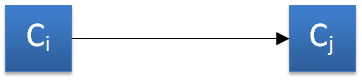
\includegraphics{figs/noNervousSystem.png}
	\caption{Relationship between the components of an organism without a nervous system.}
	\label{fig:noNervousSystem}
\end{figure}
\vspace{-0.18cm}
\paragraph{Origin of nervous systems} The evolution of nervous systems in organisms dates back to the development of primitive electrical signalling in eukaryotes, using calcium action potentials.\footnote{See any textbook on evolutionary biology.} The benefits of such mechanisms were obvious: let us imagine a microscopic organism without any sort of nervous system --- all of its behaviour is hard-coded and mechanical. It can take in nutrients through its cell walls or through an opening; parts of it can contract or expand in response to stimuli like light or pressure; homeostatic conditions can influence its chemistry. Figure~\ref{fig:noNervousSystem} shows this schema: if we enumerate the constituent parts or {\em components} of an organism as $\{C_1,\dots,C_n\}$, the organism's behavior is caused by signals being sent between $C_i$ and $C_j$ (the case $i=j$ is of course possible). Such an organism suffers from two disadvantages: (a) the behaviour is necessarily simple and (b) it is not very adaptable.

Let us now imagine that such an organism develops a bundle of cells which transmit the signals from various parts of its body, modulate them in some way, and then send them to various parts, inducing changes. Schematically, this is shown in Figure~\ref{fig:nervousSystem}, where a function $F$ is interposed between two components. The first such nervous systems were likely little more than signal transformers or magnifiers that expedited communication between parts: with a few neurons, an organism would have had the ability to coordinate movements or rely on sensing parts induce, say, movement.

\begin{figure}
	\centering
	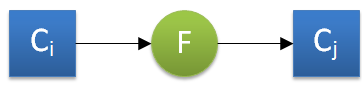
\includegraphics{figs/nervousSystem.png}
	\caption{Relationship between the components of an organism possessing a nervous system. $F$ can be understood as a simple signal transformer or a central coordinating mechanism.}
	\label{fig:nervousSystem}
\end{figure}

The neuron bundles would have been quite malleable in the face of selection pressure: when the environment required it, they could, after several generations, start to compute different or more elaborate functions. For instance, an organism which had had developed in an environment where food was abundant in bright places and which had now found itself in darkness would have benefited from a variety of plausible changes, such as
\begin{itemize}
	\item an inversion of its light-seeking behaviour,
	\item switching off its metabolism in light places to conserve energy,
	\item accelerating its metabolism in dark places to make better use of the food there.
\end{itemize}

Of course, other changes would have also been possible, such as the metabolization of different food sources,\footnote{A current-day example is given by nylon-eating bacteria, which have developed in the last century and which now have an abundant food source and no competition.} but we can see how the aforementioned three could have been effected through changes in a simple nervous system alone. Let us recall the beginning of this section and contrast such a malleable computational mesh with most products of human engineering: one cannot simply take out a piston in a car or replace a cogwheel in a mechanical clock with a differently sized one. Machines are designed to fit together perfectly and their complexity tends to be irreducible. Even programs, which are more open to mutation and which are often evolved in evolutionary algorithms, are easily broken by small changes.

\paragraph{Adaptation of nervous systems}  When discussing how an organism's nervous system can evolve and, in particular, {\em evolve to perform new tasks} and not just variations on old ones, explanations are again constrained by two criteria: (a) the change has to be small, or at least have a small cause\footnote{The effect does not have to be small --- changes in single genes can switch entire components on or off. The MYH16 gene, which is present in non-human primates but has been switched off in humans, is an example. In us, its disabling lead to a drastic reduction in the size of jaw muscles and a corresponding increase in brain size~\cite{carroll2005}.} and (b) each change must be beneficial in the short term.\footnote{Caveats apply: if the selection pressure on a group of organisms isn't too strong, changes which may be sub-optimal but perhaps beneficial at some later point may spread, and non-selective processes like genetic drift can also play a role.}

To illustrate this, we can look at a simple neural network in Figure~\ref{fig:neuralNetwork}, with a marked node $N_x$. Figure~\ref{fig:unlikelyEvolution} shows an unlikely change scenario in which some new component/function is cleanly grafted onto the system. Figure~\ref{fig:likelyEvolution} then shows a much more likely scenario: a mutation causes $N_x$ to be split and the new nodes take over some of its connections. In time, new functions can thus grow into the system, but never in the manner in which, say, an engineer would implement a new feature.

\begin{figure}
	\centering
	\begin{subfigure}[t]{0.45\textwidth}
		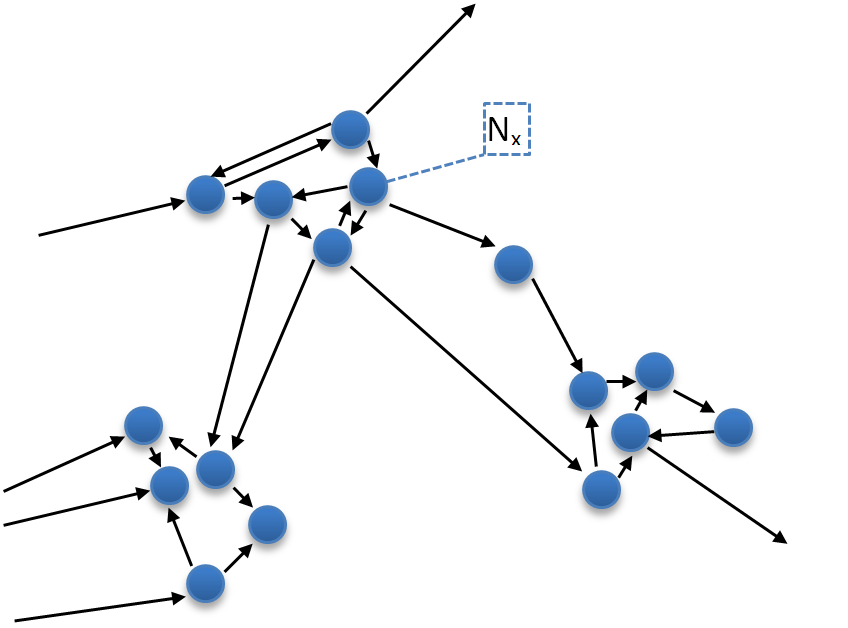
\includegraphics[width=\textwidth]{figs/neuralNetwork.png}
		\caption{A simple neural network.}
		\label{fig:neuralNetwork}
	\end{subfigure}
	\begin{subfigure}[t]{0.45\textwidth}
		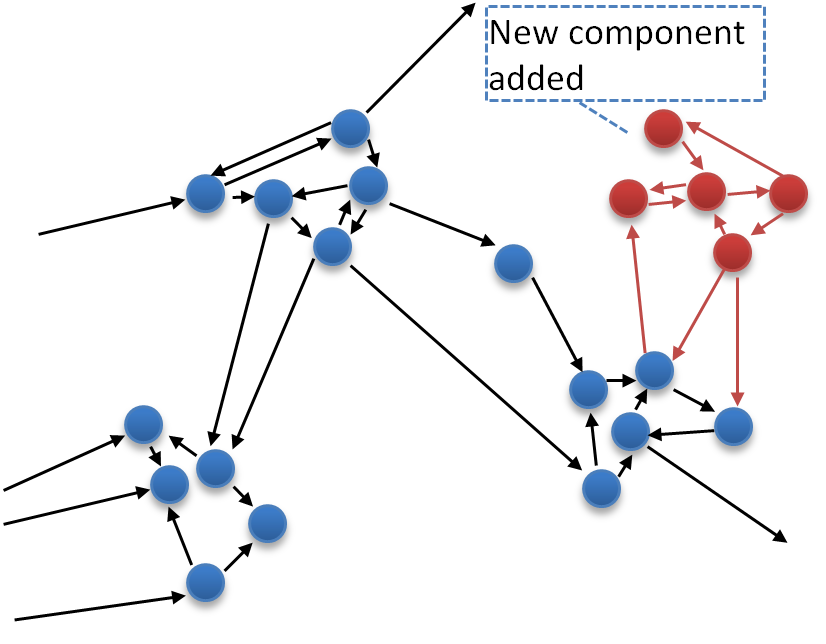
\includegraphics[width=\textwidth]{figs/unlikelyEvolution.png}
		\caption{An unlikely change scenario in which new, discernible components are grafted on from whole cloth.}
		\label{fig:unlikelyEvolution}
	\end{subfigure}
	\begin{subfigure}[t]{0.45\textwidth}
		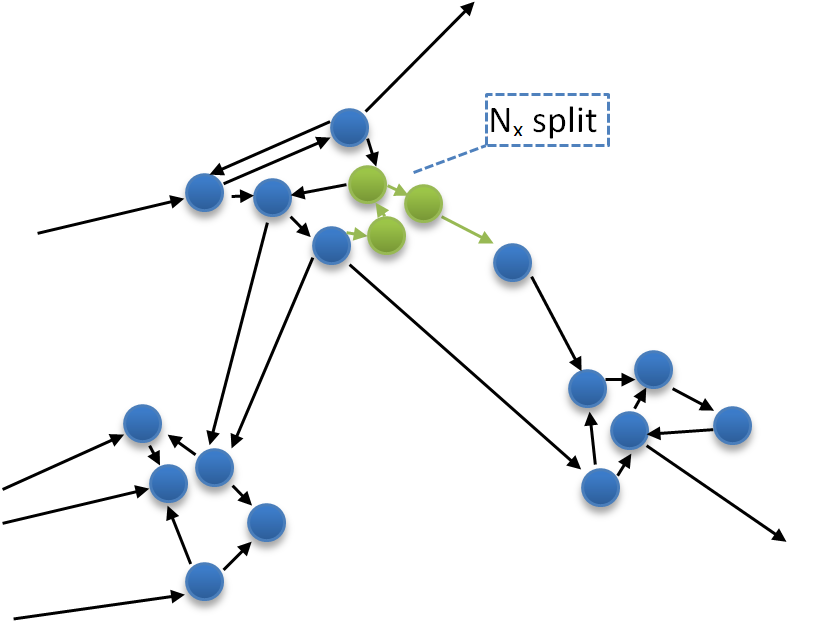
\includegraphics[width=\textwidth]{figs/likelyEvolution.png}
		\caption{A more likely change scenario in which one part is split into three but where the overall shape of the network is not appreciably altered.}
		\label{fig:likelyEvolution}
	\end{subfigure}
\end{figure}

\paragraph{The brain as a collection of functions}

The processes hitherto described are quite uncontroversial and can be found reiterated in any textbook on the evolution of nervous systems. The functional structure and the model of computation used in the brain, however, are not well understood. FMRI and similar brain imagining techniques, while invaluable, give only rough impressions about the neural correlates of certain forms of cognition and do not give fine-grained insight into its structure. As such, the model I shall describe in the following paragraphs is a conjecture. The implication of such an evolutionary viewpoint, I conjecture in this document, is that brain functions don't ``just appear'', but are rather the result of small changes and the recombination of pre-existing parts. This, in turn, informs the plausibility of various possible brain architectures. In becomes unlikely that the brain should be a collection of neatly delineated functions, or that it should have certain coordinating units or universal message formats for communication between components. The reason for this is that administrative mechanism confer little evolutionary benefit on their owen, and do not confer it gradually: the imposition of a central coordinating mechanism on a pre-existing mesh of neurons would necessitate the complete reorganisation of such, and the abandonment of the previous communication channels on favor centralized coordination. The same objections can be raised against a universal or even a local message format. Moreover, such mechanisms require substantial changes in the organism with no obvious or immediate advantage.

Such objections do not contradict the existence of macroscopic structures in the brain, dedicated to certain tasks. The development and adaptation of such remains entirely plausible. They do, however, give insight into the pattern of processing inside such structures, which is often simply regarded as atomic or replicated in computers as if it were a conventional engineering product.

Instead of a rigidly ordered brain with central organisation and large, discrete, and highly complex features like ``sight'' or ``reason'' which function like pluggable black boxes, I propose a decentralized white-box architecture composed of simple parts: first, every component, while perhaps sophisticated, is conceptually simple. Second, communication between different components is not performed in the function-call pattern of computer programs, but rather by one component listening in on the activity of another. Since there is, inherently, no mechanism of function abstraction in neural systems, it stands to reason that the most likely way for new functions to develop is for additional neurons to modulate the activity of others. In such a scheme, a visual perception component does not have to know which other components will consume its output (or rather, listen on its activity); changes which affect agent activity in useful ways based on the visual data can occur gradually and, over time, become large enough to count as components in their own right.

\paragraph{Practical abstraction}

While such a white-box model is conceptually useful, a mesh of gradually grown patterns does not lend itself to implementation in a program. Therefore, I will present a simplified model which, while attempting to remain true to the conceptual view, will, pragmatically, contain discrete functions and components. The white-box nature of brain activity will be emulated by a message-passing scheme in which messages model the internal activity of components. Instead of each component blindly acting in some fashion on the activity of another, components will have explicit parsers and interpreters and later, these will be further simplified into localized message formats and tagging, for the sake of easy implementation.

\section{Diagram notation}

In the rest of this document, a number of diagrams appear. These will use the following notation:

\begin{center}
	\begin{tabular}{p{.5\textwidth}@{}p{.4\textwidth}@{}}
		\toprule
		Symbol & Description\\
		\midrule
		
\includegraphics[width=80pt]{figs/legend_proc.png} \dotfill & Processing component\\
		
\includegraphics[width=80pt]{figs/legend_choice.png} \dotfill & Choice\\
		
\includegraphics[width=50pt]{figs/legend_container.png} \dotfill & Data container (Queue, List, etc.)\\
		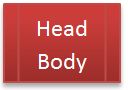
\includegraphics[width=50pt]{figs/legend_data.png} \dotfill & Data\\
		
\includegraphics[width=30pt]{figs/legend_generator.png} \dotfill & Stream generator\\
		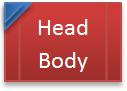
\includegraphics[width=50pt]{figs/legend_imaginary.png} \dotfill & Counterfactual (imaginary) data\\
		\bottomrule
	\end{tabular}
\end{center}

\section{Global architecture}\label{sec:globalArchitecture}

We can imagine the components of the mind as white boxes which inform other components by their very functioning --- however, this does not lend itself to easy implementation. Instead, we can emulate this behaviour via a \caps{message space}, from which individual components take their input and into which they put their output. A \caps{component} is then a local processing unit which continuously scans the message space, running messages through its \caps{filter}. If the filter detects a relevant message, it is then passed to the \caps{interpreter}, which parses the message into the needed format and hands it over to the \caps{processor}. The processor, after having finished, puts its output back into the message space for other other components to read. Figure~\ref{fig:global} illustrates this scheme. Note the lack of explicit hierarchical structure and central organising units.

\begin{figure}[!h]
	\centering
	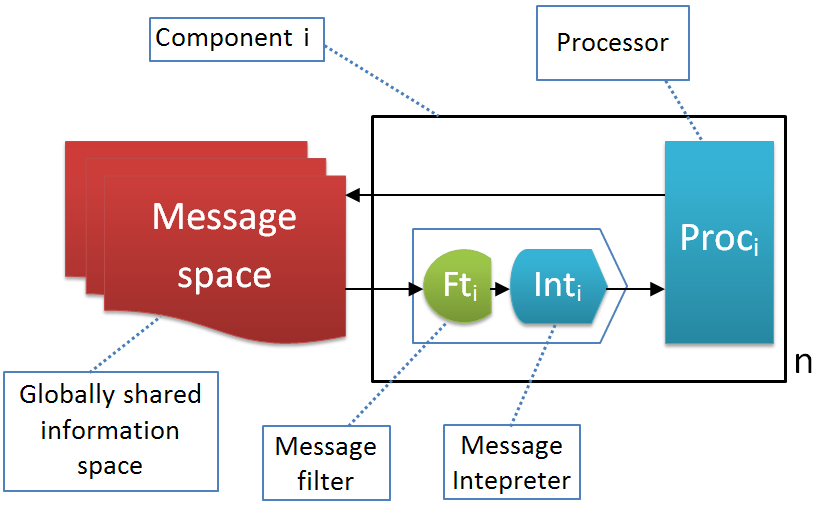
\includegraphics[width=400pt]{figs/global.png}
	\caption{Global neural architecture.}
	\label{fig:global}
\end{figure}

However, as I'll show in the next section, this model is generic enough to accommodate such special-purpose structures. Figure~\ref{fig:global} shows the message-passing scheme, but it also specifies a graph in which the nodes are the components and fixed, while the edges are the accepted messages and are determined by the nodes; through their filters, components control the shape of the graph. By imposing invariants on these filters, we can have the graph take any shape we desire. In particular, we can model the kinds of structures that occur in many other cognitive models and in empirical research: central organisers, sequences of components (``pipelines''), localized messages affecting only a small part of the mind, a component reading its own messages, loops and iterative messages between two or more components et cetera.

\pagebreak

\paragraph{Messages}

We may now ask how such messages between components are structured. Here, I make two empirical claims:
\begin{enumerate}
	\item messages have a priority and
	\item they are effectively unstructured.
\end{enumerate}

\begin{figure}[!h]
	\centering
	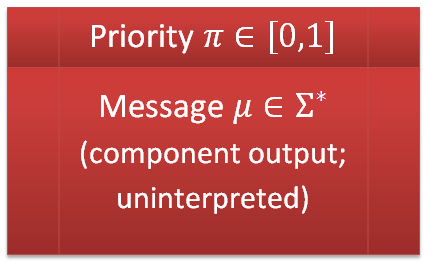
\includegraphics[width=150pt]{figs/message.png}
	\caption{Structure of a neural message.}
	\label{fig:message}
\end{figure}

To the best of my knowledge, the veracity of either has thus far not been determined by neuroscience. For the first, Marvin Minsky's ``The Emotion Machine'' provides some circumstantial evidence \cite[p. 222]{emotionMachine}:

\begin{quote}
	Of course, when one activates two or more Critics or Selectors, this is likely to cause some conflicts, because two different resources might try to turn on a third resource both {\em on} and {\em off}. To deal with this, we could design the system to use various policies like these:
	
	\begin{enumerate}
		\item Choose the resource with the highest priority.
		\item Choose the one that is most strongly aroused.
		\item Choose the one that gives the most specific advice.
		\item Have them all compete in some ``marketplace''.
	\end{enumerate}
\end{quote}

The selection strategies Minsky lists imply that there is some mechanism in the brain to determine the urgency of a signal. While it is possible that higher brain functions like reasoning or affect make an additional, rational evaluation, sensations like intense pain, bright lights, or great sadness can likely be communicated most easily by the appropriate components causing a flood of activity which, by its very intensity, informs other components of the urgency of their messages.

The second claim --- that messages are essentially unstructured --- means that there is no common, agreed-upon format in which they are stored. In addition to the evolutionary implausibility of such a format being created, an unstructured message format is in line with the white-box nature of components: since components merely ``listen in'' on others, and since each components will have its own pattern of activity, a listener would simply have to try and make sense of this activity as best it could. The proposed structure of messages is thus shown in Figure~\ref{fig:message}: every message comprises a priority header, together with an unstructured body which, for our purposes, is simply a string of bits.

\paragraph{Filters} Before a component can respond to a message by another, such a message must be assessed for the presence of relevant information. Conceptually, this happens via a \caps{filter} in each component, which pattern-matches incoming messages and, if a certain threshold is reached, signals relevance and hands the message over the \caps{interpreter} for parsing. Figure~\ref{fig:filter} shows such a filter: it is composed of a directed graph of nodes, and a node is activated if it detects some specific content in the message. Nodes, in turn, are connected via edges of strength $\in [0,1]$. When a node is activated, it sends a charge proportional to the strength of its link to its neighbours, contributing to their activation as well. Some nodes are marked as {\em output nodes}; if enough such output nodes become activated, the message is deemed to be sufficiently relevant. This model of filters is inspired by the {\em spiking neural P Systems} of Georghe Pa\u{u}n et al. (\cite[p. 337]{membraneComputing} and \cite{spikingNeural}), in which charges sent along directed graphs of neurons are used to compute functions.

\begin{figure}[!h]
	\centering
	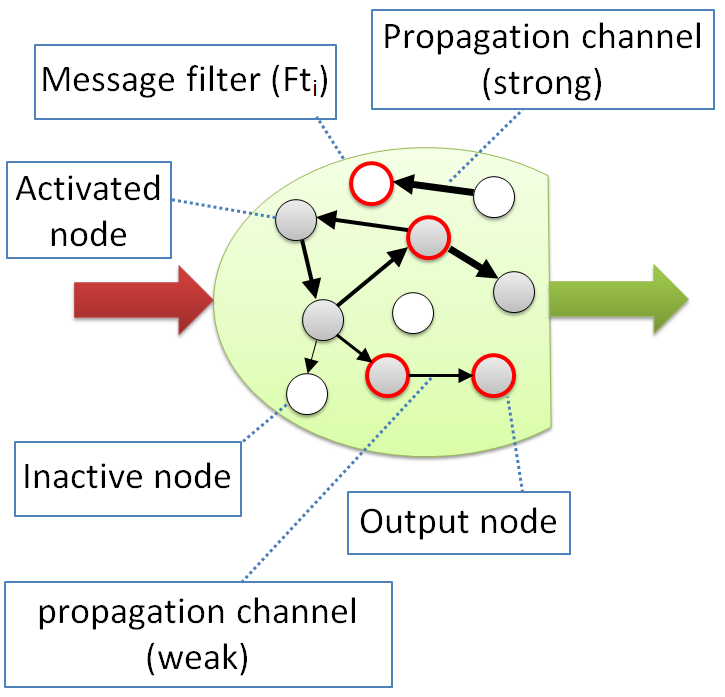
\includegraphics[width=215pt]{figs/filter.png}
	\caption{A pattern-matching filter for a component $C_i$.}
	\label{fig:filter}
\end{figure}

\section{Schema of cognition}\label{sec:schemaOfCognition}

We can imagine the components of the mind as white boxes which inform other components by their very functioning --- however, this does not lend itself to easy implementation. Instead, we can emulate this behaviour via a \caps{message space}, from which individual components take their input and into which they put their output. A \caps{component} is then a local processing unit which continuously scans the message space, running messages through its \caps{filter}. If the filter detects a relevant message, it is then passed to the \caps{interpreter}, which parses the message into the needed format and hands it over to the \caps{processor}. The processor, after having finished, puts its output back into the message space for other other components to read. Figure~\ref{fig:global} illustrates this scheme. Note the lack of explicit hierarchical structure and central organising units.

\begin{figure}[!h]
	\centering
	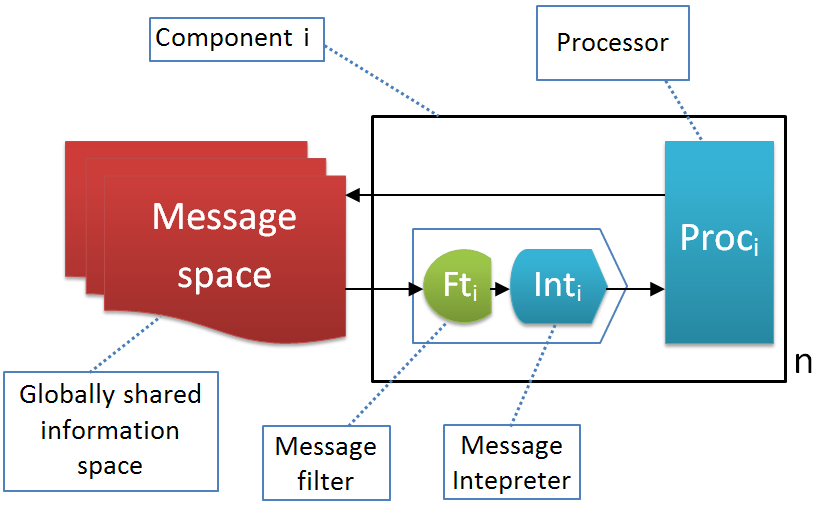
\includegraphics[width=400pt]{figs/global.png}
	\caption{Global neural architecture.}
	\label{fig:global}
\end{figure}

However, as I'll show in the next section, this model is generic enough to accommodate such special-purpose structures. Figure~\ref{fig:global} shows the message-passing scheme, but it also specifies a graph in which the nodes are the components and fixed, while the edges are the accepted messages and are determined by the nodes; through their filters, components control the shape of the graph. By imposing invariants on these filters, we can have the graph take any shape we desire. In particular, we can model the kinds of structures that occur in many other cognitive models and in empirical research: central organisers, sequences of components (``pipelines''), localized messages affecting only a small part of the mind, a component reading its own messages, loops and iterative messages between two or more components et cetera.

\pagebreak

\paragraph{Messages}

We may now ask how such messages between components are structured. Here, I make two empirical claims:
\begin{enumerate}
	\item messages have a priority and
	\item they are effectively unstructured.
\end{enumerate}

\begin{figure}[!h]
	\centering
	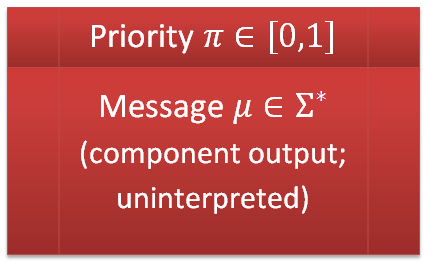
\includegraphics[width=150pt]{figs/message.png}
	\caption{Structure of a neural message.}
	\label{fig:message}
\end{figure}

To the best of my knowledge, the veracity of either has thus far not been determined by neuroscience. For the first, Marvin Minsky's ``The Emotion Machine'' provides some circumstantial evidence \cite[p. 222]{emotionMachine}:

\begin{quote}
	Of course, when one activates two or more Critics or Selectors, this is likely to cause some conflicts, because two different resources might try to turn on a third resource both {\em on} and {\em off}. To deal with this, we could design the system to use various policies like these:
	
	\begin{enumerate}
		\item Choose the resource with the highest priority.
		\item Choose the one that is most strongly aroused.
		\item Choose the one that gives the most specific advice.
		\item Have them all compete in some ``marketplace''.
	\end{enumerate}
\end{quote}

The selection strategies Minsky lists imply that there is some mechanism in the brain to determine the urgency of a signal. While it is possible that higher brain functions like reasoning or affect make an additional, rational evaluation, sensations like intense pain, bright lights, or great sadness can likely be communicated most easily by the appropriate components causing a flood of activity which, by its very intensity, informs other components of the urgency of their messages.

The second claim --- that messages are essentially unstructured --- means that there is no common, agreed-upon format in which they are stored. In addition to the evolutionary implausibility of such a format being created, an unstructured message format is in line with the white-box nature of components: since components merely ``listen in'' on others, and since each components will have its own pattern of activity, a listener would simply have to try and make sense of this activity as best it could. The proposed structure of messages is thus shown in Figure~\ref{fig:message}: every message comprises a priority header, together with an unstructured body which, for our purposes, is simply a string of bits.

\paragraph{Filters} Before a component can respond to a message by another, such a message must be assessed for the presence of relevant information. Conceptually, this happens via a \caps{filter} in each component, which pattern-matches incoming messages and, if a certain threshold is reached, signals relevance and hands the message over the \caps{interpreter} for parsing. Figure~\ref{fig:filter} shows such a filter: it is composed of a directed graph of nodes, and a node is activated if it detects some specific content in the message. Nodes, in turn, are connected via edges of strength $\in [0,1]$. When a node is activated, it sends a charge proportional to the strength of its link to its neighbours, contributing to their activation as well. Some nodes are marked as {\em output nodes}; if enough such output nodes become activated, the message is deemed to be sufficiently relevant. This model of filters is inspired by the {\em spiking neural P Systems} of Georghe Pa\u{u}n et al. (\cite[p. 337]{membraneComputing} and \cite{spikingNeural}), in which charges sent along directed graphs of neurons are used to compute functions.

\begin{figure}[!h]
	\centering
	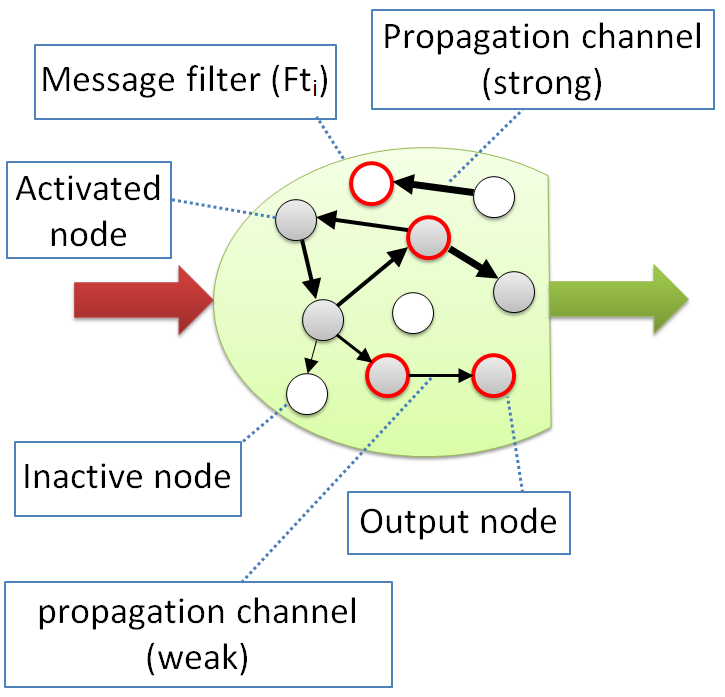
\includegraphics[width=168pt]{figs/filter.png}
	\caption{A pattern-matching filter for a component $C_i$.}
	\label{fig:filter}
\end{figure}

\section{Mathematical model}\label{sec:mathematicalModel}

We now create a mathematical model for the description of the architecture of Section~\ref{sec:globalArchitecture}. This model will be split into two parts: the structural and the operational semantics. The structural semantics encode the static properties of neural systems, whereas the operational semantics describe the behaviour of such a system at runtime.

\subsection{Preliminaries}\label{sec:mathematicalPreliminaries}

Since the mathematical model is built with implementation in mind, I will use some basic type theory in the coming sections. In this section the relevant notions will be introduced, without assuming any prior knowledge about the topic.

\begin{definition}[Syntax: Type]\label{def:type}
For our purposes, types are defined inductively thus:
	\begin{description}
		\item[Basic type.] $\N$, $\R$, and $\emptyset$ are types.
		\item[Sum type.] If $\type{T_1},\type{T_2}$ are types, the sum type $\type{T_1 + T_2}$, is a type. 
		\item[Product type.] If $\type{s}$ is a string and $\type{T_1},\dots,\type{T_n}$ are types, the product type $\type{s}\ \type{T_1} \dots \type{T_n}$, is a type. A special case is the {\em anonymous product type} \paren{tuple}, where $s=``\langle\rangle"$. There, we just write $\langle\type{T_1},\dots,T_n \rangle$.
		\item[Full application.] If $\type{T_1},\dots,\type{T_n}$ are types and $\allQ{x_1,\dots,x_n} \type{C}$ is a type constructor \paren{see next definition}, then $\type{C\ T_1} \dots \type{T_n}$, is a type.
	\end{description}
\end{definition}

\begin{definition}[Syntax: Type constructor]\label{def:typeCon}\
	Type constructors are the defined thus:
	\begin{description}
		\item[Base case.] Every type $\type{T}$ is a type constructor.
		\item[Abstraction.] If $\type{C}$ is a type constructor and $\type{T}$ is a type, $\allQ{x} \type{C}[\type{T}\backslash x]$ is a type constructor.
		\item[Sum types.] If $\type{C_1}\dots,\type{C_n}$ are type constructors with $\type{C_i} = \allQ{x^i_1\dots,x^i_n} \type{T_i}$ \paren{$1 \leq i \leq n$}, then\\ $\allQ{x_1,\dots,x_n} (\type{C_1} + \dots + \type{C_n})$ is a type constructor.
		\item[Partial application.] If $\type{T_1},\dots,\type{T_i}$ \paren{$i < n$} are types and $\allQ{x_1,\dots,x_n} \type{T}$ is a type constructor,\\ then $\allQ{x_{i+1},\dots,x_n} \type{T}[x_1\backslash \type{T_1},\dots,x_i\backslash \type{T_i}]$ is a type constructor.
	\end{description}
\end{definition}

Every type is simply interpreted as a set of values which are of that type; type constructors are interpreted as universally quantified templates for actual types. Their formal semantics are as follows:

\begin{definition}[Semantics: Type]\label{def:typeSem}
Let $\type{T}$ be a type. Its interpretation function $\tint(\type{T})$ is defined thus:.
	\begin{description}
		\item[Basic type.] $\N$ and $\R$ are interpreted as the natural and real numbers, respectively. $\tint(\emptyset) = \{\}$.
		\item[Sum type.] If $\type{T_1}, \type{T_2}$ are types, then $\tint(\type{T_1 + T_2}) = \tint(\type{T_1}) \cup \tint(\type{T_2})$.
		\item[Product type.] If $\type{T_1},\dots,\type{T_n}$ are types and $\type{s}$ is a string, then
		$$
			\tint(\type{s}\ \type{T_1} \dots \type{T_n}) = \left\{
				\begin{array}{l l}
					\{\type{s}\} & \mt{if } n = 0\\
					\{\type{s}\} \times \tint(\type{T_1}) \times \dots \times \tint(\type{T_n}) & \mt{if } n \geq 1.
				\end{array}
			\right.
		$$
		
		\item[Full application.] If $\type{T_1},\dots,\type{T_n}$ are types and $\allQ{x_1,\dots,x_n} \type{C}$ is a type constructor, then
		$$
			\tint(\type{C}\ \type{T_1} \dots \type{T_n}) = \bigcup\limits_{v_1 \in\ \tint(\type{T_1})} \cdots \bigcup\limits_{v_n \in\ \tint(\type{T_n})} \left( \bigcup\limits_{C' \in\ \cint(C)} C'[x_1\backslash v_1,\dots, x_n\backslash v_n] \right).
		$$
	\end{description}
\end{definition}

\begin{definition}[Semantics: Type constructor]\label{def:typeConSem}
The partial interpretation function $\cint$ for type constructors is defined as follows: if $\type{C}$ is a type constructor containing exactly the types $\type{T_1},\dots,\type{T_n}$, then
	$$
		\cint(\type{C}) = \bigcup\limits_{v_1 \in\ \tint(\type{T_1})} \cdots \bigcup\limits_{v_n \in\ \tint(\type{T_n})} \type{C}[\type{T_1}\backslash v_1,\dots,\type{T_n}\backslash v_n].
	$$
\end{definition}

Intuitively, sum types are simply unions, product types are named cartesian products, and full applications are instantiations of type constructors with all possible values. Type constructors themselves are just generic types.

Whenever we want to assert that an expression has a specific type, we write:

\begin{notation}[Typed expressions]
	Let $x$ be an expression and $\type{T}$ a type. $x :: \type{T}$ asserts that $x$ has type $\type{T}$.
\end{notation}

Henceforth, by convention, we will write type variables in lower-case and concrete types in upper-case, omitting the explicit $\forall$-blocks. That is, a type like $\allQ{x,y,z} \type{C\ x\ (\N + T_1)\ y\ z}$ will simply be written as $\type{C\ x\ (\N + T_1)\ y\ z}$ and it will be clear that $\type{x}, \type{y}, \type{z}$ are type variables, while $\N, \type{T_1}$ are concrete types. A special kind of type constructor is the function arrow ($\rightarrow$) which induces the function type:

\begin{example}[Function arrow]
	If we take, say, the type $\rightarrow \type{S1}\ \type{S2}$ (a product type with the product types $\type{S1}$ and $\type{S2}$ as arguments) and abstract twice, we get $\allQ{s,t} \rightarrow \type{s}\ \type{t}$. $\rightarrow \type{s}\ \type{t}$ is the type constructor for unary functions from $\type{s}$ to $\type{t}$, also written infix as $\type{s} \rightarrow \type{t}$. Functions with multiple arguments, mapping $\type{t_1},\dots,\type{t_{n-1}}$ to $\type{t_n}$, can be modelled in two ways: either through n-tuples, or through nested function arrows:
	
	$$
		\begin{array}{l}
			\tuple{\type{t_1}, \type{t_2}, \dots \type{t_{n-1}}} \rightarrow \type{t_n}\\
			\type{t_1} \rightarrow (\type{t_2} \rightarrow \dots \rightarrow (\type{t_{n-1}} \rightarrow \type{t_n})\cdots)
		\end{array}
	$$
	
	The first method necessitates that we supply all arguments at once, whereas the second allows them to be given one after another.
\end{example}

\noindent
Function arrows allow the execution of functions in the obvious way:

\begin{definition}[Function application]
	Let $f :: \type{S} \rightarrow \type{T}$ and $x :: \type{T}$ Then $f(x) :: \type{T}$.
\end{definition}

\noindent
We can combine type constructors, sum types, and product types into {\em algebraic data types} (ADTs).

\begin{definition}[Algebraic data type (ADT)]\label{def:ADT}
Let $\type{s}$ be a string and $\type{C_1},\dots,\type{C_n}$ be type constructors such that $\type{C_i} = \allQ{x_1,\dots,x_n} \type{T_i}$ and $\type{T_i}$ is a named product type with type variables \paren{$1 \leq i \leq n$}. Then $\allQ{x_1,\dots,x_n} (\type{T_i} + \dots + \type{T_n})$ is an ADT. If we want to give a name to an ADT, we write it as $\type{s\ x_1 \dots x_n = T_i + \dots + T_n}$.
\end{definition}

Since an ADT is merely the sum of product types, it is itself a type constructor. If it has no type variables, it is also a type. Next, we define a couple of example ADTs, some of which we will use in the next section.

\begin{example}[$\B$, $\Q$, $\C$,  Maybe, Either, List]
	$$
		\begin{array}{l c l}
			\B & = & \type{False + True}\\
			\Q & = & \type{Rat}\ \N\ \N\\
			\C & = & \type{Complex}\ \R\ \R\\
			\type{Maybe\ t} & = & \type{Nothing + Just\ t}\\
			\type{Either\ l\ r} & = & \type{Left\ l + Right\ r}\\
			\type{[]\ a} & = & \type{[] + (a : [a])}\\
		\end{array}
	$$
	
	Here, $\type{False}$, $\type{True}$, $\type{Nothing}$, and $\type{[]}$ are nullary product types; $\type{Left}$, $\type{Right}$ are unary type constructors \paren{which can be instantiated into unary product types}. ``:'' is a binary type constructor, written infix. $\type{Rat}\ \N\ \N$ and $\type{Complex}\ \R\ \R$ are binary product types.\\
	
	$\B$, $\Q$, $\C$ are the sets of Boolean number and rational/complex numbers, respectively. $\mathtt{Maybe}$ represents an optional value, which may or may not be present. $\mathtt{Either}$ represents a choice between two values, of which either the left or the right one is present, but not both. $\type{[a]}$ denotes a list of values of type $\type{a}$.
\end{example}


Definitions~\ref{def:type}--\ref{def:ADT} specify a fragment of System F$_\omega$,\footnote{Specifically, the decidable fragment of System F$_\omega$ without higher kinds and only prenex-polymorphism. That is, type constructors can only take types as arguments and are of the form $\allQ{x_1,\dots,x_n} \type{C}$ for quantifier-free $\type{C}$. This is also called the Hindley-Milner type system. For details, see Barendregt \cite{barendregt91}.} which is used to type expressions in the lambda calculus. Although System F$_\omega$ is strictly more powerful, our definitions are enough to provide a description language for the data types and functions in the rest of this work.


\subsection{Neural systems}\label{sec:mathematicalNeuralSystem}

\begin{definition}[Neural component]
	Let $I$ be an index set and let $\type{T}$ be any type. Then, a neural component $C$ with a name from $I$ and message type $\type{T}$ is a four-tuple
	$$
		\tuple{\field{name}, \field{ft}, \field{int}, \field{proc}}
	$$
	where
	\begin{enumerate}
		\item $\field{name} :: I$ is the {\em name} of $C$,
		\item $\field{ft} :: \type{T \rightarrow \B}$ is  called the {\em filter} of $C$,
		\item $\field{int} :: \type{T} \rightarrow \type{Maybe\ T}$ is called the {\em interpreter} of $C$, and
		\item $\field{proc} :: \type{T} \rightarrow \type{T}$ is called the {\em processor} of $C$.
	\end{enumerate}
	
	Formally, the type of $C$ is $\field{Comp}_{\type{T},I}$. As a shorthand, we denote the name, filter, interpreter and processor of a given component $C$ as $\field{name}_C$, $\field{ft}_C$, $\field{int}_C$, $\field{proc}_C$, respectively.
\end{definition}

\noindent
A set of neural components, together with a set of messages, induces a {\em neural system}:

\begin{definition}[Neural system]
	Let $T$ be any type and let $I$ be an index set. Then, a neural system with message type $T$ and component names from $I$ is a tuple
	$$
		\langle \textbf{Co}, \textbf{Me} \rangle
	$$
	where
	\begin{itemize}
		\item $\textbf{Co}$ is a set of neural components (with message type $T$ and names from $I$) and
		\item $\textbf{Me}$ is a set of elements of type $T$, called the {\em set of messages}.
	\end{itemize}
\end{definition}

\subsection{Sending and receiving messages}\label{sec:notation}

We now give a notation for the sending and receiving of messages in a system. Here, we distinguish two aspects: first, the structural, which describes how messages {\em can} travel in a system and the operational, which describes how they {\em do} travel in some given scenario.

\subsubsection{Structural notation}

The elements of a component statically determine which messages it can receive and send. Based on the behaviour of the filter, interpreter and processor of a component, we can express a number of properties.

\begin{definition}[Message reception]
	Let $C$ be a component and $m$ a message. $C$ can receive $m$ if and only if $\ft{C}(m) = \field{True}$ and $\int{C} = \field{Just } m'$ for some $m'$.
	When $C$ can receive all messages in $\{m_1,\dots,m_n\}$, we write:
	$$
		\canrec{m_1,\dots,m_n}{C}.
	$$
	
	We denote the opposite statement --- that $C$ cannot receive any message in $\{m_1,\dots,m_n\}$ --- by:
	
	$$
		\cantrec{m_1,\dots,m_n}{C}.
	$$
\end{definition}

\begin{definition}[Message sending]
	Let $C$ be a component and $m, m_1,\dots,m_n$ messages. $C$ can send out a message $m$ if and only if there exists a message $m_{\mt{in}}$ s.t. $\proc{C}(m_{\mt{in}}) = m$.
	When $C$ can send all messages in $\{m_1,\dots,m_n\}$, we write:
	
	$$
		\cansend{C}{m_1,\dots,m_n}.
	$$
	
	The opposite statement --- that $C$ cannot send any message in $\{m_1,\dots,m_n\}$ --- is again denoted by:
	$$
		\cantsend{m_1,\dots,m_n}{C}.
	$$
\end{definition}

\begin{definition}[Receiving set]
	The set of components which can receive a message $m$ is denoted by
	
	$$
		\rec{m} \equiv \{C \in \co\ |\ \canrec{m}{C} \}.
	$$
	
	$\field{rec}$ can also be overloaded to refer to the set of components which can receive and interpret at least some message of a component $C$:
	
$$
	\rec{C} \equiv \{C_i \in \co\ |\ \exists m:\ \cansend{C}{m} \wedge \canrec{m}{C_i} \}.
$$
\end{definition}


\subsubsection{Operational notation}

Whereas the structural notation pertained to the static properties of a neural system, the operational notation describes {\em traces}: lists of sent and received messages, and the changes they induced in the system.

\begin{definition}[Message action]
	When a component $C_i$ outputs a message $m_{out}$ that another component $C_j$ receives and interprets as message $m_{in}$, we write
	
	$$
		C_i \rightarrow [m_{out}, m_{in}] \rightarrow C_j.
	$$
	
	We refer to this as {\em message action}. If it's clear that the message $m$ does not change, we just write
	
	$$
		C_i \rightarrow [m] \rightarrow C_j.
	$$
\end{definition}

\begin{definition}[Trace]
	Traces are defined inductively thus:
		\begin{enumerate}
			\item Every message action is a trace.
			\item If $T_1$ and $T_2$ are traces, $T_1;T_2$ is a trace.
		\end{enumerate}
		
	``$;$'' denotes sequential execution and is associative. Thus, the semantics of a trace $T_1;T_2;\dots;T_n$ are that $T_1$ is executed first, followed by $T_2$, and so forth, until $T_n$ is reached and the execution ends.
	For readability, $T_1;\dots;T_n$ will sometimes be written line-by-line as
	$$
		\begin{array}{l}
		T_1\\
		\vdots\\
		T_n
		\end{array}
	$$
\end{definition}

\begin{definition}[Component mutation]
	Let $f_1,f_2,\dots$ be functions $\compT{T}{I} \rightarrow \compT{T}{I}$ which preserve the names of components, $m,m'$ messages of type $T$, and let $C$ be a component of type $\compT{T}{I}$. When $C$ is changed into $f_n \circ \dots \circ f_1 (C)$ by a message $m$ it receives, or changed into $f_n \circ \dots \circ f_1 (C)$ by a message $m'$ it sends, we write, respectively:
	$$
		\begin{array}{c}
			\dots \rightarrow [m] \rightarrow \langle f_1,\dots,f_n \rangle C\\
			C\langle f_1,\dots,f_n \rangle \rightarrow [m'] \rightarrow \dots
		\end{array}
	$$
	
	\noindent
	If no change occurs, that is, if
	$$
		\begin{array}{r l}
			C\langle\rangle \rightarrow [m] \rightarrow \dots & \mt{or}\\
			\dots \rightarrow [m] \rightarrow \langle\rangle C
		\end{array}
	$$
	
	\noindent
	we omit the angle brackets.
	The semantics are as follows: after by sending or receiving a message, $\co$ is replaced by $(\co - \{C\}) \cup \{f_n \circ \dots \circ f_1 (C) \}$.
\end{definition}

\begin{definition}[Plastic and non-plastic neural systems]
	If, for all messages $m$ and components $C, C'$ in a neural system, the following holds:
	$$
		C\langle\rangle \rightarrow [m] \rightarrow \langle\rangle C'
	$$
	
	\noindent
	we call the system non-plastic. Otherwise, we call it plastic.
\end{definition}


This definition intends to roughly convey the notion of neuroplasticity, as used in neuroscience: areas in the brain are changed over time through specific patterns of activity. Here, such change is modelled by the execution of functions and the replacement of $C$ in the system by $f_n \circ \dots \circ f_1 (C)$.

\subsection{Invariants}

Such a model does not necessitate the existence of special structures, such as central organizers or sequences of components, one activated after another,\footnote{An example of such a sequence is found in \cite{DBLP:journals/nn/SanderGS05} where the authors model the emotion process as a four-step pipeline of relevance, implication, coping and normative significance.} but it does not preclude them either. In fact, we can enforce certain features via first-order invariants. For example, a central organizing units for the components $C_1,\dots,C_n$ can be emulated by a component $C_{co}$ which accepts messages and transforms them into an appropriate format for the some other components.

\begin{invariant}[Central organiser]
$$
	\begin{array}{l}
	 [\forall i \in \{1\dots,n\}] [\forall m]:\\
	 \quad \quad \left(\cansend{C_i}{m} \Rightarrow \rec{m} = \{C_{co}\}\right) \wedge \left( \left( \proc{C_{co}} \circ \int{C_{co}}(m)  \right) \in \bigcup\limits_{1 \leq j \leq n} \rec{C_j} \right).
	\end{array}
$$
\end{invariant}

Figure~\ref{fig:centralOrganizer} depicts such an organizer. Similarly, sequences can be created by components $C_{1},\dots,C_{n}$, where each components reads the message of the last one.

\begin{invariant}[Sequence]
$$
	[\forall i \in \{2\dots,n\}]:\ \rec{C_{i-1}} = \{C_i\}.
$$
\end{invariant}

\begin{figure}
	\centering
	\begin{subfigure}[t]{0.45\textwidth}
		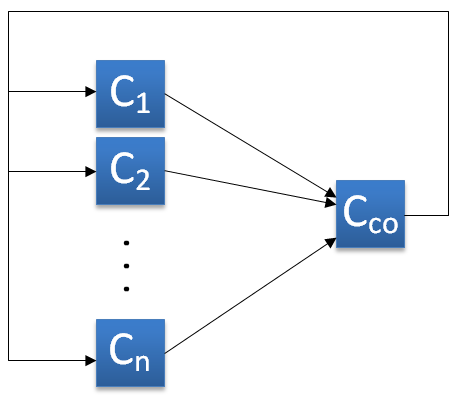
\includegraphics[width=\textwidth]{figs/c_co.png}
		\caption{Components communicating via a central organising mechanism.}
		\label{fig:centralOrganizer}
	\end{subfigure}
	\begin{subfigure}[t]{0.45\textwidth}
		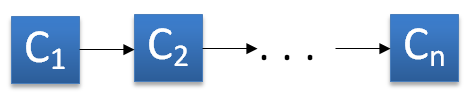
\includegraphics[width=\textwidth]{figs/c_sequence.png}
		\caption{A sequence of components.}
		\label{fig:c_sequence}
	\end{subfigure}
\end{figure}

\section{Selected subsystems}\label{sec:selectedSubsystems}

The global architecture now specified, we will introduce three related subsystems and fit them into this global framework: sensory perception --- the processing of raw sensory input into an format intelligible to other brain components ---, counterfactual perception --- the imagination, which mimics the output of the senses ---, and affect --- broadly speaking, the emotional component of cognition.

\subsection{Sensory perception}\label{sec:sensoryPerception}

The model presented herein is inspired by Marvin Minsky's ``The Emotion Machine''. Therein, Minsky proposes a layered mental structure where each successive layer operates on more and more abstract representations of the world, starting with primitive sensations and proceeding all the way to self-conscious reflection and rational planning. Figure~\ref{fig:brainLayers} shows such a layered structure.

 \begin{figure}[!h]
 	\centering
 	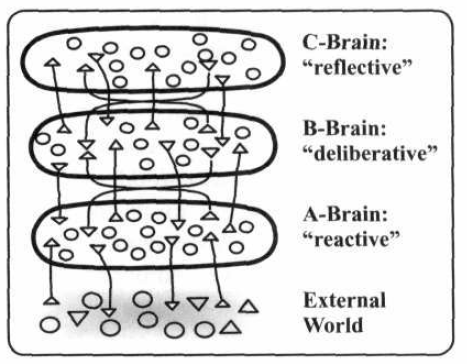
\includegraphics[width=300pt]{figs/emotionMachine_brainLayers.png}
 	\caption{Layered perception of the world, from \cite[p. 100]{emotionMachine}.}
 	\label{fig:brainLayers}
 \end{figure}
 
 \newpage
 
The diagram is explained thus \cite[p. 100]{emotionMachine}:

\begin{quote}
	Now suppose that your A-Brain gets some signals from the external world (via such organs as eyes, ears, nose, and skin) --- and that it also can react to these by sending signals that make your muscles move. By itself, the A-Brain is a separate animal that only reacts to external events but has no sense of what they might mean. For example, when the fingertips of two lovers come into intimate physical contact, {\em the resulting sensations, by themselves, have no particular implications}. For there is no significance in those signals themselves: their meanings to those lovers {\em lie in how they prepresent and process them in the higher levels of their minds.}
\end{quote}

If we apply this to the architecture of Section~\ref{fig:global}, we can devise a system in which each sense $S$ has an associated component $C_S$ which does two things:
\begin{enumerate}
	\item Consume the raw sensory information delivered by various organs and output processed input for higher brain functions;
	\item as a side a effect of this processing, cause  instinctive, low-level reactions in the body, such as pulling away from pain or jumping at a sudden fright.
\end{enumerate}

In Figure~\ref{fig:sensoryPerception}, a slice of just such a system is shown for visual, auditory, olfactory/gustatory and tactile sensation. The produced data can be of two kinds: one is more abstract than the input and facilitates deliberative action, and the other contains instructions for instinctive behaviour for the body.

\begin{figure}[!h]
	\centering
	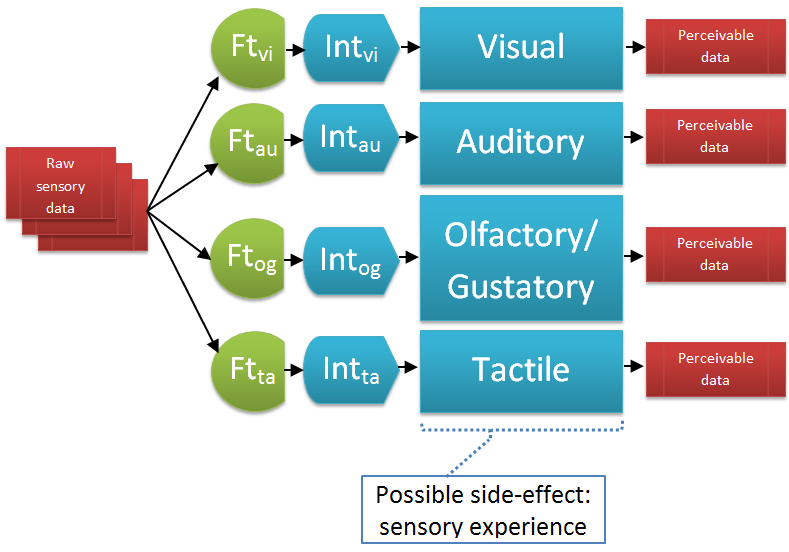
\includegraphics[width=325pt]{figs/sensoryPerception.png}
	\caption{Partial structure of sensory perception - raw sensory data is processed and made available to higher functions such as the affective subsystem. The comment ``Possible side-effect: sensory experience'' signifies the fact that conscious and sub-conscious sensory experiences might occur as a side-effect of this processing. However, it is currently unknown to neuroscience whether this is indeed the case.}
	\label{fig:sensoryPerception}
\end{figure}


\subsection{Counterfactual perception and planning}\label{sec:worldSimulation}

Broadly speaking, counterfactual perception can be described as ``imagination'', and is closely related to sensory perception and world simulation. In examining the system, we might broadly classify its processes into three categories:

\begin{enumerate}
	\item Counterfactual perception --- imagining sights, sounds, etc. Such experiences have much in common with those caused by our sensory organs, yet are marked not as real. In particular, imagined experiences evoke only parts of the conscious experience that accompanies real perceptions. Research by Berthoz and Lotze et al.\ suggests that (a) the brain indeed uses similar circuitry for real and imagined experiences and that (b) imagined experiences are prevented from being confused with real ones via inhibitory signals. Lotze et al.\ write \cite{lotze1999}:
	\begin{quote}
		The results of cortical activity support the hypothesis that motor imagery and motor performance possess similar neural substrates. The differential activation in the cerebellum during EM and IM is in accordance with the assumption that the posterior cerebellum is involved in the inhibition of movement execution during imagination.
	\end{quote}
	
	From the abstract of Berthoz's paper \cite{8713551}:
	
	\begin{quotation}
		(...) experimental evidence suggesting that the brain can use the same mechanisms for the imagination and the execution of movement. In particular the fact that adaptation of the vestibulo-ocular reflex can be obtained by pure mental effort and not solely by conflicting visual and vestibular cues has been suggestive of the fact that the brain could internally simulate conflicts and use the same adaptive mechanisms used when actual sensory cues were in conflict.
	\end{quotation}
	
	\item World simulation --- the imagination of future states. Simulating worlds goes beyond the imagination of sensory experiences; it involves constructing models of worlds and simulating their behaviour. The details of this process are unknown, but we can assert that it is capable of a number of things:
	\begin{enumerate}
		\item construction of non-physical worlds, such as mathematical models,
		\item extrapolation into the future and the past
		\item simulation of the minds itself and other agents.
	\end{enumerate}
	
	
	\item Executive planning --- humans can plan both both in immediate and concrete terms (such as body movement) and in the abstract. It is likely that different circuitry is used for movement planning and for planning involving abstract reasoning, in both cases it is necessary that the brain simulate the world in some way. The simulation of the consequences of body movement is likely older than humanity and distinct from the kind of world simulation described above, but both share their function: the agent proposes as series of actions to take, inserts them into some mental world and judges the utility of those actions based on the predicted consequences.
\end{enumerate}

Needless to say, that this process in all its subtleties is immensely complex and thus I simply endeavour to sketch its possible structure only in extremely rough outlines. This sketch is shown in Figures~\ref{fig:imagination},  \ref{fig:planner}, and \ref{fig:worldSimulatorPlannerInteraction}: the world simulation is an ordinary component with a filter and interpreter which outputs, for simplicity's sake, messages marked as counterfactual. We can imagine such messages to be very much like ordinary sensory ones, with the exceptions that they have no accompanying sensation and, more importantly, that we are aware of their non-reality. The planning component receives instructions about desirable states and outputs hypothetical actions which the world simulator incorporates. The world simulator's output is in turn read by the planner, which then abandons the plan or decides to pursue it further.

\begin{figure}
	\centering
	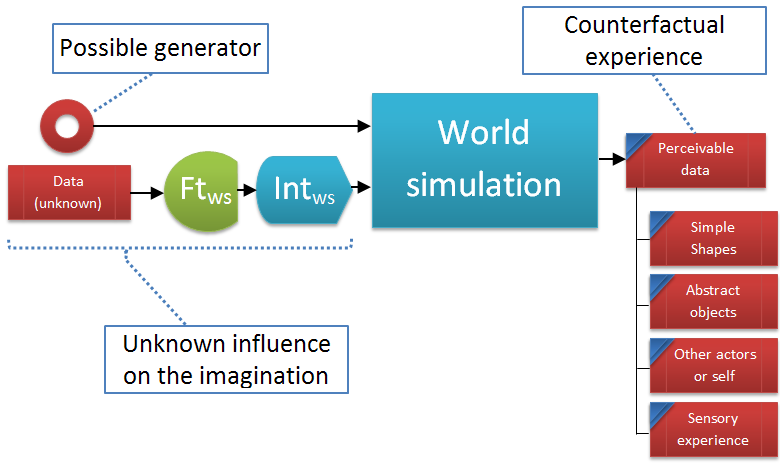
\includegraphics[width=\textwidth]{figs/imagination.png}
	\caption{Structure of of counterfactual perception \& world simulation: messages emulating the output of sensory perception are generated, but are marked as counterfactual by unknown means.}
	\label{fig:imagination}
\end{figure}

\begin{figure}
	\centering
	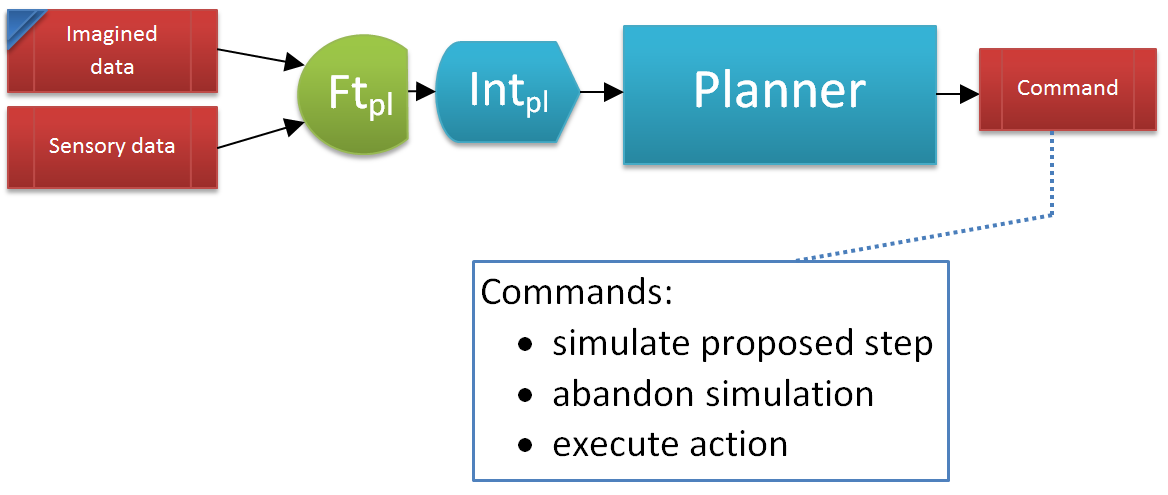
\includegraphics[width=\textwidth]{figs/planner.png}
	\caption{Planner with two kinds of inputs: (1) real sensory data and (2) counterfactual data which comes from world simulation. On the basis of these inputs, possible steps are developed and sent out as commands.}
	\label{fig:planner}
\end{figure}

The planner, minimally, has to perform two functions --- first, it has to judge the desirability of various world states and second, it has to be able to devise possible steps for the agent based on some strategy. If these two functions and some desired goal(s) are given, the planner can do its work by issuing the following commands, as shown in Figure~\ref{fig:planner}:
\begin{enumerate}
	\item If some goals are not yet reached but appear possible, devise possible steps to take and have the world simulator predict their outcomes.
	\item If the goals appear impossible the necessary steps prohibitively undesirable, command the world simulator to cease its activity.
	\item If earlier proposed steps turn out to fulfil some goal, contact the agent's executive component.
\end{enumerate}

\begin{figure}
	\centering
	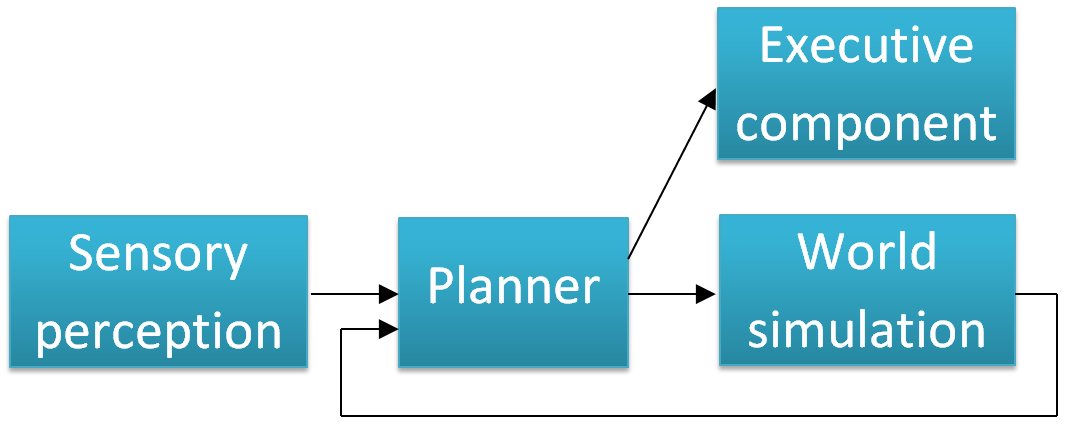
\includegraphics[width=\textwidth]{figs/worldSimulatorPlannerInteraction.png}
	\caption{Interaction between world simulator and planner: the planner devises possible steps and feeds them into the world simulator, which, in turn, tries to calculate their effects. The results are fed back to the planner.}
	\label{fig:worldSimulatorPlannerInteraction}
\end{figure}

\subsubsection{World simulation as rationality}
The way in which I just described the interaction between the world simulator and the planner suggests that they function as a pair of guesser and checker: the planner generates ideas on what to do and the world simulation tests their viability in some setting. Indeed, we can model rational thinking as embedded in the world simulator, especially if we make use of a plastic neural system. The proposed steps of the planner might be quite chaotic and irrational, but when given to the world simulator, it recognises them as such and returns a failure signal to the planner, causing it to abandon ``bad'' paths of cognition. A plastic planner can learn from the consistent failure of certain kinds of steps and, in time, propose them less and less often. Observed as a whole, this system of planner and simulator appears to simply deliver good plans by intuition, even though, in isolation, neither part is very clever.\footnote{I do not wish to idealize rationality too much; world simulation is only partly rational and, given faulty information about the world, will err considerably and in documented ways. Similarly, it is certainly possible for the planner to derange the world simulator by evaluating certain states as so desirable/undesirable that it will pursue even scenarios which the world simulator reports as highly unlikely.}

\paragraph{Model.} In a simplified way, we can model the process of logical deduction in a formal system $F = (A, R)$, where $A$ is a recursive set of axioms and $R$ is a recursive set of production rules of the form $(r_{\mt{from}}, r_{\mt{to}})$ s.t. $r_{\mt{from}} \rightarrow r_{\mt{to}}$ is a valid production in the system. Let
	\begin{enumerate}
		\item $W$ be a world simulator for the world of propositions $\mathcal{P}$ in $(A,R)$,
		\item $P$ a planner,
		\item $\mathrm{St} = \{s_1,\dots,s_p\}$ a set of messages about steps to take,
		\item $\mathrm{Cat} = \{K_1,\dots,K_q\}$ a list of message categories,
		\item $\field{cur} : W_S$ the current state of the world simulator,
		\item $\field{ins} :: W_S \rightarrow \mathrm{St} \rightarrow W \rightarrow W$, $\field{del} :: \mathrm{St} \rightarrow W \rightarrow W$ functions for inserting or deleting a state change into the world simulator or the planner,
		\item $t(i)$ and $b(i)$ functions which increase or decrease the likelihood of sending a message belonging to category $K_i$ and 
		\item $\bot_{i}, \top_{i}$ the failure and success signals of a message belonging to the category $K_i$.
	\end{enumerate}
	
One step of the interaction between $W$ and $P$, in a scenario where $P$ proposes steps $s_{i_1},\dots,s_{i_n}$, can then be modelled with two traces $T_{\mt{guess}}$ and $T_{\mt{check}}$:

$$
	\begin{array}{l l l}
		T_{\mt{guess}}(\tt{step}) & \equiv & \sendsf{P}{\tt{ins cur step})}{\tt{step}}{\tt{step}}{\tt{ins cur step})}{W}\\
		\\
		T_{\mt{check}}(\tt{step}) & \equiv &
		\forall K_i \in Cat: K_i(\tt{step}) \Rightarrow\\
		
		& & \hspace{1cm} \mt{if } \exQ{s_j} (\field{cur}, s_j) \in R\ \mt{ then } \
					\sendsf{W}{}{\top_i}{\top_i}{t\ i}{P}\\
		& & \hspace{1cm} \mt{else }\ \sendsf{W}{\tt{del step})}{\bot_i}{\bot_i}{\tt{del step}, b\ i}{P}\\
	\end{array}
$$

\medskip

Axioms can be selected by executing $T_{\mt{guess}}(\tt{ax})$ for all $\tt{ax} \in A$. We can then perform deduction via $T_{\mt{guess}};T_{\mt{check}}$, for a probabilistically selected $\tt{step} \in St$.

Intuitively, $T_{\mt{guess}}$ guesses a step to take. It does so but inserting it into the planner's world-state via $\tt{ins}$ and then sending a message to the world simulator, which also inserts it into its world state. $T_{\mt{check}}$ then checks whether the change from $\tt{cur}$ to $\tt{step}$ was legitimate. If so, it determines to which category $\tt{step}$ belongs and sends the $\top$-signal for that category back to the planner. Otherwise, it sends the corresponding $\bot$-signal. The purpose of this is to make it more or less likely, respectively, that the planner should choose the same category of step in the future. The categories, we can imagine, could be things like ``modus ponens'', ``associative reasoning'', ``appeal to consequences'' and so forth.

If we repeat this interaction (with different proposed steps $s_1,\dots,s_p$ in each iteration), we get an algorithm for logical deduction  --- that is, since $A$ and $R$ are recursive, the system will recursively enumerate all valid logical formulas, provided that we pursue each path and that the probability of selecting any valid step is $> 0$. In addition, we could add a goal function $g$ to $P$ s.t. it would accept certain states and stop. Thereby, $P$ and $W$ could be used to prove logical propositions.

\subsection{Affect}\label{sec:affect}

When discussing human affect, one can mean various things: the causation of emotion, its internal mechanisms, the expression of emotion, social communication of emotions, etc. In this document, we restrict our attention just to the internal mechanisms --- that is, to the means by which emotions are evoked in an agent and how they shape its thinking.

Furthermore, the issue will only be the causative mechanism itself; taxonomy and hierarchy of emotions are deferred to future versions of this document.

The model presented herein is adapted from Gadanho and Hallam \cite{DBLP:journals/adb/GadanhoH01}, who employed it in the context of robot learning. They constructed a system of \caps{feelings} and \caps{sensations} $\mathcal{F}$, \caps{emotions} $\mathcal{E}$, and a hormone storage $H$.

\begin{figure}[!h]
	\centering
	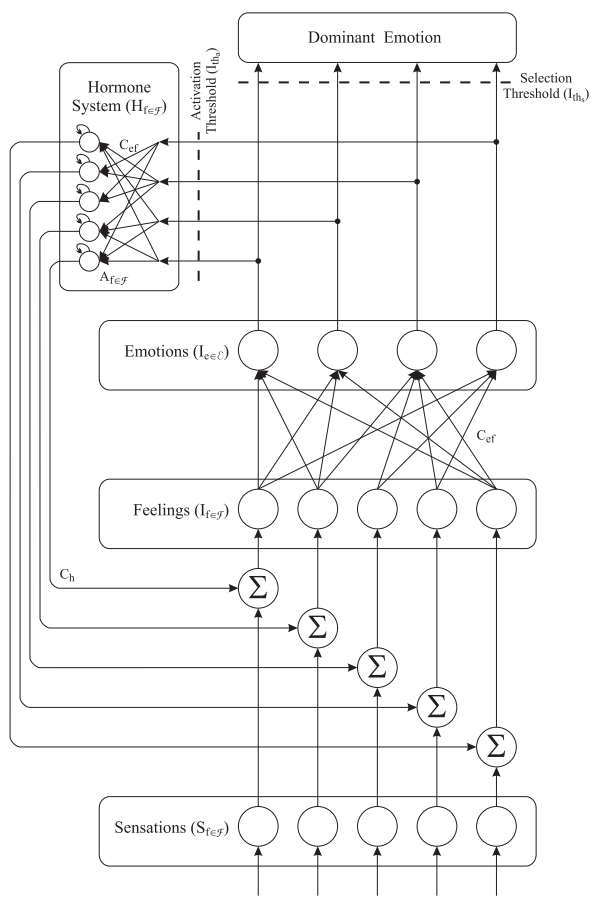
\includegraphics[width=200pt]{figs/gadanhoModel.png}
	\caption{Emotional model of Gadanho and Hallam \cite[p. 46]{DBLP:journals/adb/GadanhoH01}.}
	\label{fig:gadanhoModel}
\end{figure}

Figure~\ref{fig:gadanhoModel} shows this model: \caps{sensations} enter the system and are connected to the \caps{feelings}. They, in turn, determine the agent's \caps{emotions}. The emotions then feed into a \caps{hormone storage}, the contents of which influence, together with the \caps{sensations}, the agent's \caps{feelings}. In the context of their paper, this model had a very restricted application. Its purpose was to merely help guide a robot through a world, and accordingly, $\mathcal{F}$ and $\mathcal{E}$ were only defined as \cite[p. 47]{DBLP:journals/adb/GadanhoH01}:
$$
	\begin{array}{l}
		\mathcal{F} = \{ \mt{Hunger}, \mt{Pain}, \mt{Restlessness},
						 \mt{Temperature}, \mt{Eating}, \mt{Smell},
						 \mt{Eating}, \mt{Proximity} \}\\
		\mathcal{E} = \{ \mt{Happiness}, \mt{Sadness}, \mt{Fear},
						 \mt{Anger} \}
	\end{array}
$$

\begin{figure}[!h]
	\centering
	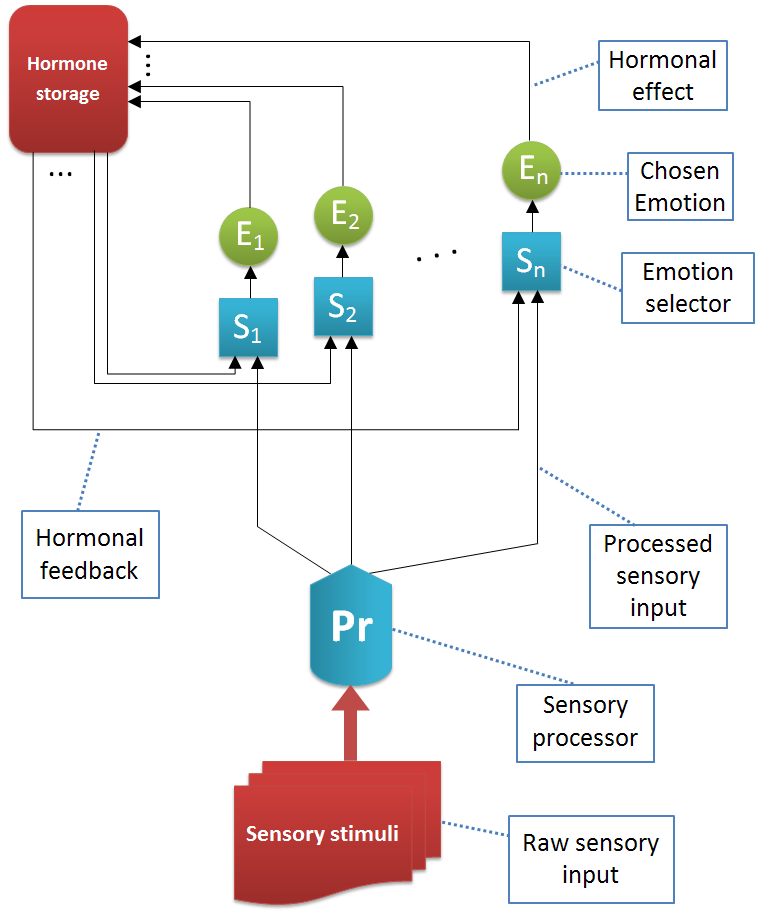
\includegraphics[width=400pt]{figs/affectiveSubsystem.png}
	\caption{Affective subsystem; specialisation of the global neural architecture. In plastic neural systems, selections may change over time.}
	\label{fig:affectiveSubsystem}
\end{figure}

\pagebreak
The main advantage of Gadanho's and Hallam's model is that (a) it is sufficiently generic to accommodate various schemas and (b) posits an internal state (the hormone storage), giving agents a certain inertia. For example, one can imagine integrating a many-dimensional model like Brazeal's \cite{breazeal2003} detailed taxonomy of emotion like Ortony's OCC model \cite{ortony1988}. The existence of an internal state is necessitated by the simple observation that our internal world is not solely dependent on momentary stimuli, but merely influenced by them. The idea of a hormone storage might be a simplistic approximation but it, too, can be refined as needed.\footnote{It might be tempting to simply replace the hormone storage with the message space, but doing so would ignore the role that neurotransmitters like dopamine and serotonin play in cognition, irrespective of the purely computational activity of brain components.} Figure~\ref{fig:sensoryPerception} shows the adapted model. The general structure was retained, but the set of sensations was replaced by the sensory processor described in Section~\ref{sec:sensoryPerception} and, instead of a single dominant emotion, competing emotions simply emit messages which are used by execute components and the world simulation.

\subsubsection{Affective subsystems}

In this section, I will develop the concept of ``emotion'' in greater detail. The process shown in Figure~\ref{fig:affectiveSubsystem} might suggest we simply have a collection of emotions and that all emotions are essentially equal, but I submit that this is not so. Instead, I propose the existence of various subsystems, each responsible for a group of emotions, and each with its own history and distinctive tasks. In the rest of this work, the following two assumptions will be made:

\begin{enumerate}
	\item {\em ``Emotion'' is not a singular phenomenon.} Specifically, this is contradicts many-dimensional models of emotions which propose one, two, three or four axes and a corresponding vector space in which every emotion is a point. Such a view implies that all emotions share a neurological template which is parametrized with coordinates to result in different experiences.
	\item {\em There exist emotions which are both different in kind and which pertain to different subsystems in the brain.} This implies that emotions cannot morally be seen as a homogeneous set $\{E_1,\dots,E_n\}$. Instead, a number of distinct subsystems are necessitated, each responsible for the causation and processing of a group of emotions. Given this, the only substantial aspect any two emotions might have in common would be our referring to both of them as ``emotion''.
\end{enumerate}

Both of these assumptions are rather concrete and thus deserve evidence. In 1999, Davidson and Irwin, using PET and fMRI scanning, found two different systems mediating approach- and avoidance related behaviors \cite[p. 13]{davidson1999}:

\begin{quote}
A large body of lesion, neuroimaging and electrophysiological data supports the view that the prefrontal cortex (PFC) is an important part of the circuitry that implements both positive and negative affect. ($\dots$)
A number of early studies that evaluated mood subsquent to brain damage suggested that patients with damage to the left hemisphere, particularly in PFC, were more likely to develop deppressive symptoms compared with patients having lesions in homologous regions of the right hemisphere. ($\dots$)
The general finding of left dorso-lateral PFC damage increasing the likelihood of deppressive symptoms has been interpreted to reflect the contribution of this cortical territory to certain features of positive affect, which, when disrupted, increases the probability of depressive symptomatology.
\end{quote}

In this, they echo earlies findings by Cacioppo et al.\ \cite{cacioppo1999}, Gray \cite{gray1994} and Lang et al.\ \cite{lang1990} that affect is lateralized, with different hemispheres being responsible for different categories of feeling. It therefore stands to reason that different emotions, being generated by different brain regions, should therefore also be different in their character.

Further, much research has been done in the area of so-called {\em basic emotions} --- a small set of emotions are acknowledged as being both elementary and characteristically distinct from each other. The Cambridge Handbook of Affective Neuroscience provides a good overview of the basic emotion theory \cite[pp. 9-10]{cambridgeAff}. Matsumoto and Eckman \cite{matsumoto2009}, for instance, identified seven basic emotions: happiness, surprise, contempt, sadness, fear, disgust, and anger.

Damasio \cite{damasio1998}, drawing upon neuroscientific findings, sketches a model of affect mainly involving the prefrontal cortex, but also the amygdala, the hypothalamus, and the anterior cingulate cortex, as seen in Figure~\ref{fig:damasioSystem}.

\begin{figure}
	\centering
	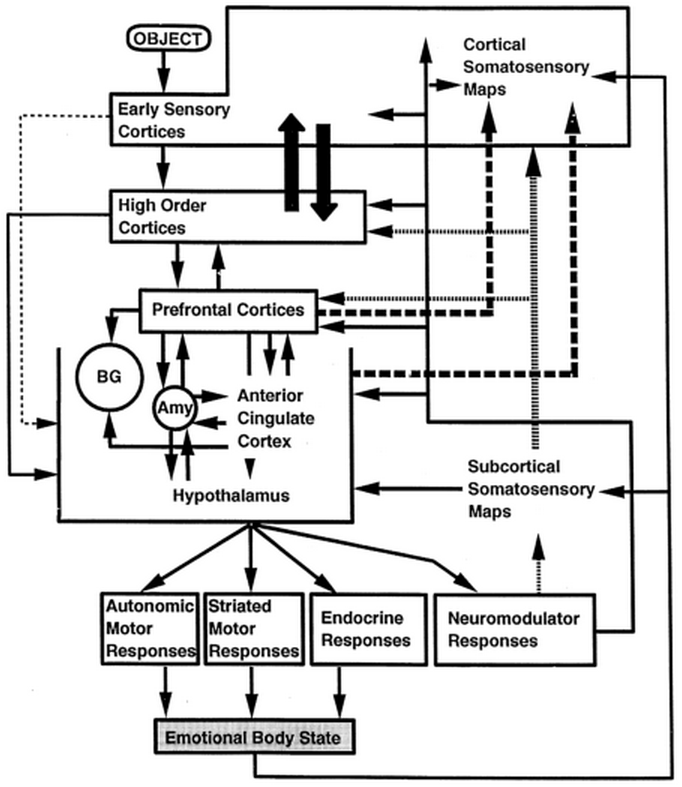
\includegraphics[width=250pt]{figs/damasioSystem.png}
	\caption{Neurological structure of affect, according to Damasio \cite{damasio1998}.}
	\label{fig:damasioSystem}
\end{figure}

In the same article, he describes how different brain regions are responsible for different kinds of emotion:

\begin{quotation}
	Equally problematic is the widespread view that the limbic system is the neural basis for all emotions. A rich body of evidence tells us that this is just not the case. Both within and around the limbic system, circuitry connection varied neural sites supports the operation of different emotion. For instance, work on aversive conditioning in rodents has shown that the amygdala is certainly involved in negative emotions such as fear [10,6]. {\em Work in humans, on the other hand, has not only confirmed the amygdala's involvement in negative emotions such as fear and anger, but also shown that the amygdala is not involved in the processing of positive emotions such as happiness, or negative emotions such as disgust.} [emphasis mine]
\end{quotation}

The last sentence of that quotation is especially revealing: it states that the neurological distinction is not simply one between positive and negative, or one between approach- or avoidance-related emotions, but that each emotion has its own profile of neurological activity and involves its own peculiar set of brain structures.

These facts make it quite clear that emotions are not simply homogeneous phenomena, being induced by a single system in the brain; rather, they are different in character and in the neural structures they involve. 

\paragraph{Structure of affect} The system depicted in Figure~\ref{fig:affectiveSubsystem} left several parts unspecified: the sensory processor $\Pr$, the emotion selectors $S_1,\dots,S_n$ and the messages sent by the chosen emotions into the message space. In the following paragraphs, I will flesh out that model in greater detail, building principally on the work of Sander, Grandjean and Scherer \cite{DBLP:journals/nn/SanderGS05}. Sander and colleagues partitioned the emotion process into four stages, as shown in Figure~\ref{fig:sanderSystem}. The first is {\em relevance}, which functions as a filter and detects the intrinsic pleasantness and the level of (emotional) attention that a stimulus demands. The processes of this stage, roughly speaking, correspond to the work of the sensory processor $\Pr$. The second stage is {\em implication}, where reasoning becomes engaged in order to determine the cause, likely outcome, and urgency of the perceived facts. At this stage, emotions like joy, anger, contentment, disgust, etc. are evoked, together with approach- and avoidance-related behaviours --- this corresponds to the emotion selectors $S_1,\dots,S_n$. Deliberate strategies come only in the next stage: {\em coping}. In it, reasoning and planning become fully engaged. The fourth stage is {\em normative significance} and deals, in essence, with moral concerns, both internal and those of other agents.

\begin{figure}
	\centering
	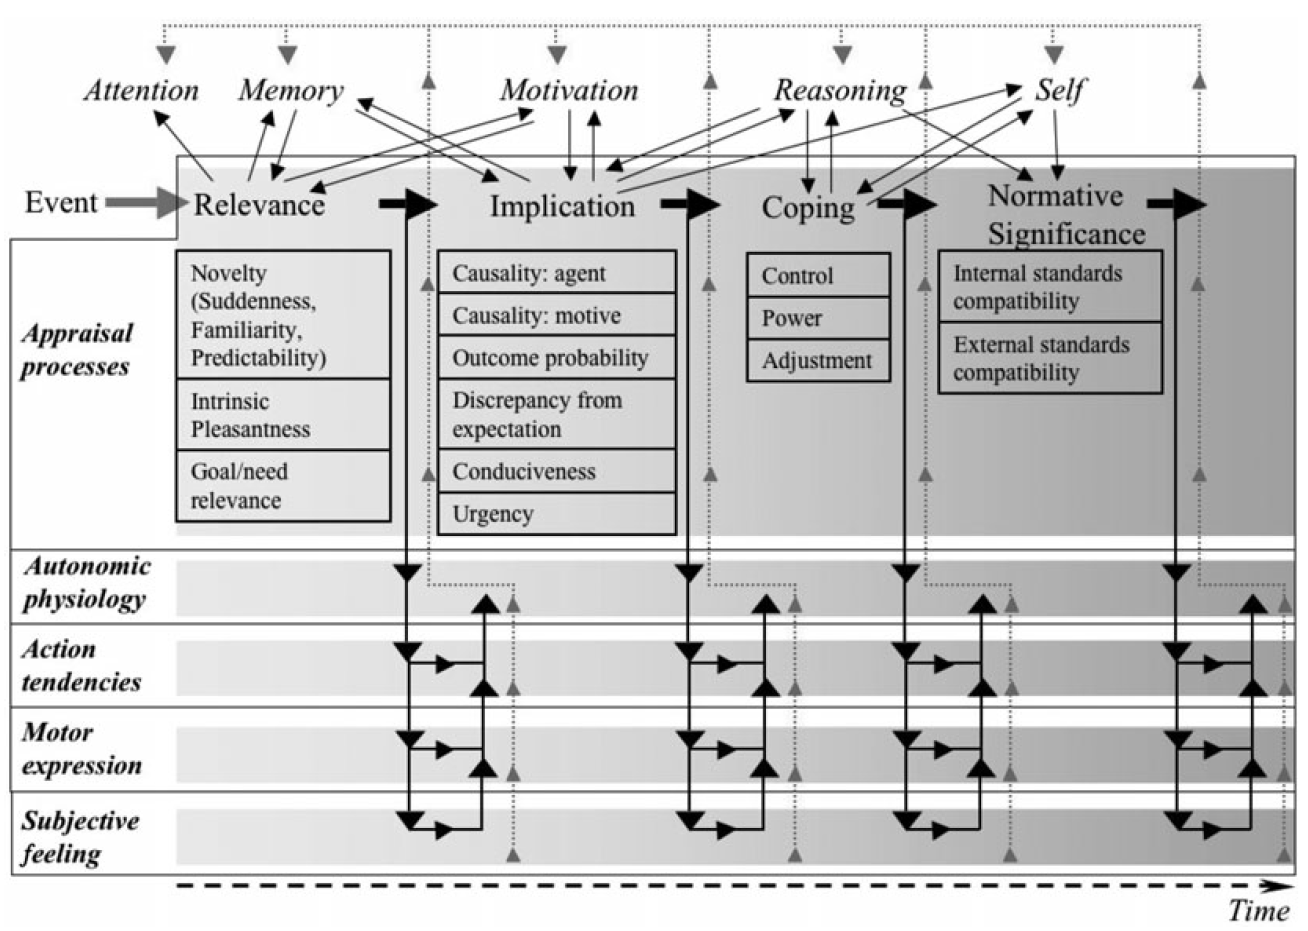
\includegraphics[width=440pt]{figs/sanderSystem.png}
	\caption{The four-stage emotion process according to Sander et al, consisting of relevance, implication, coping and normative significance.}
	\label{fig:sanderSystem}
\end{figure}

Sander et al.\ give a good, detailed account of the interactions of affect with other systems, although I would argue that theirs is unduly suggestive of a simple {\em pipeline}., rather than a mesh of systems into which the affective ones are embedded. In addition, it does not address the interactions with perception, memory, and reasoning. Based on the evidence discussed above, I shall now present a more horizontal view and construct a model of the hypothesized emotional subsystems and their interactions with other parts of the brain. Since no established vocabulary seems to exist in this specific are I shall first introduce a number of terms.

\begin{definition}[Evocative system]
An evocative system is a subsystem in the brain responsible for evoking consciously experienced affect within an agent based on internal or external stimuli.
\end{definition} 

Various such evocative systems can be imagined. I propose the following rough categorization:

\begin{description}
	\item[Pre-social emotions.] Certain behavioural mechanisms can be observed in non-social as well as social animals. The flight-or-flight instinct, for example, is nearly universal, as is the inclination to seek out food, shelter, and other resources. ``Instinct'' is indeed a more appropriate term in the case of most species, rather than ``emotion'', which connotes a certain richness of experience. Nonetheless, we can clearly see that, in more intelligent, social animals, emotions like anger, fear, and joy, have grown out of just these instincts. Hence the term ``pre-social emotions'': while emotion itself is quite possibly inherently social, certain emotions are rooted in instincts which are not, and an emotional animal would feel them even if it were the only one of its kind in an environment.
	
	\item[Social emotions.] A by far richer subset of emotions are the social ones. Indeed, social situations are the ones where affect can and must truly shine: the presence of other individuals the entire tribe demand a variety of affect relating to the appraisal of the agents, sympathy/antipathy, respect/contempt, the appraisal of oneself, showing dominance or submission, influencing other group members, taking action as a group, judging the behaviour of agents against norms, etc. It is also in social emotions in which it even makes sense to {\em show} emotion: facial expressions and gestures provide the signalling and mechanism needed for group coherence and coordinated action.
	
	We can identify several subsystems in the category of social emotion:
	
	\begin{enumerate}
		\item Reflective judgement about oneself in relation to the group or to abstract norms, primarily pride and shame \cite{Teroni2008}, but possibly also jealousy and humiliation (which, in contrast to shame, is attributed to external causes) \cite{fontaine2009};
		\item other-related judgement which determines whether to feel sympathy or antipathy, compassion, respect or contempt, trust or distrust for other individuals;
		\item normative judgement, which determines whether others or oneself is acting in accordance with instinctive or cultural norms.
	\end{enumerate}
	
	Other classifications are also possible. Haidt \cite{haidt2003}, for example, identifies those that are other-condemning (disgust, contempt), self-conscious (shame, embarrassment), other-suffering (compassion), other-praising (gratitude, awe). The picture is immensely complex and the neurological structure is presently not known. For the purposes of this thesis, we will therefore content ourselves with only this roughest of outlines.
	
	\item[Aesthetic emotions.] This type of emotion is perhaps the least studied in neuroscience and AI. It is certainly the most subtle and the least ``utilitarian'' type --- as such, it is philosophers, rather than AI researchers, who study it. For instance, Jenefer Robinson, in {\em Deeper Than Reason: Emotion and Its Role in Literature, Music, and Art} \cite{robinson2005}, writes about the affective appraisal of artwork as an unconscious process which partly reproduces the emotions of its creator. In this, she builds upon and modifies Collingwood's 1983 {\em The Principles of Art} \cite{collingwood1938, SEPcollingwood}. Since aesthetics are not the focus of this work, I shall leave it at this mention. A more thorough exploration would be interesting future work, however.
\end{description}

The emotions just listed can all be found in the more extensive taxonomies, chiefly among them in Ortony's OCC model \cite{ortony1988}. The taxonomies, however, tend to neglect the underlying neurology and the chronology of the development of these systems. Ortony's classification specifically is persuasive up to a point, but, despite it being fine-grained, one is left wondering about the underlying structure: which emotions are caused by the same brain regions, what structure, if any, do two given emotions share, to what degree is the classification scheme isomorphic to the actual neurology? This is an active area of research and while these questions are interesting, we have to leave them largely open for now.

The evoked feelings tie into and directly influence the agent's actions. This includes conscious, deliberate ones, such as avoiding an unsympathetic person, but also sub-conscious ones and those that are purely internal, such as the focusing one's attention to an important topic. These actions all fall under the umbrella term of {\em executive system}:

\begin{definition}[Executive system]
An executive system is a subsystem in the brain which makes decisions about the behaviour of an agent's mind or muscular system.
\end{definition}

This definition leaves open what exactly a decision is.In principle, any neural activity in a part of the brain could be seen as a decision of sorts, since it influences neural activity in other parts. While we do perceive certain processes as deliberate and others as automatic, this is simply what our introspection tells us and does not reflect the underlying reality; (conscious) decision-making is as mechanical as any other process in the brain, the chief difference being that we are aware of the workings of that process and perceive the control it exerts over cognition as coming from us.\footnote{I should add that we are not even aware of the entirety of our decision-making. This is especially apparant when we are asked to make trivial or random choices. A person who is asked to press a left or a right button, for example, will choose one at seemingly random, but will not be explain why one button was chosen over another. Moreover, there is evidence that the choice is made before the person {\em knows} that a choice was made: Soon et al. \cite{soon2008} instructed subjects to press a button and to record when they through they made the decision to do so. Brain scanning revealed spikes in the activity of the lateral and medial frontopolar cortices and the posterior cingulate contex {\em before} the subjects claimed their decisions were made. In effect, they only became aware of their supposedly free decisions after they had already been made. From their conscious perspective, the decision simple ``popped into their heads''.}

Nonetheless, there are properties by which we can identify executive systems in the brain: on a sufficiently high level of abstraction, we can see that certain components are receptive to control signals. Certain other components --- these are the executive systems --- have as their {\em chief purpose} the the sending of such control signals. The former accomplish some conceptually small task and essentially serve as building blocks. The latter structure the work and assemble the small building blocks into compound actions. See Section~\ref{sec:worldSimulation}, where planner and world simulator work in tandem, with the world simulator bearing the workload and the planner having control.

We can now distinguish certain kinds of action. While those performed with the ``body'' (i.e. the skeletomuscular system) are the most visible ones, we, as shown, also make decisions regarding the contents of our minds --- we decide {\em what to think about}. We then add the distinction between consciously and sub-consciously made actions and get the following four categories of executive system:

\begin{description}
	\item[Sub-conscious motor control.] instinctive reaction, such as the jerking away from pain, jumping when startled, and turning towards interesting visual stimuli;
	\item[Conscious motor control.] deliberate, planned action which the agent experiences as a choice;
	\item[Sub-conscious mental control.] involuntary but consciously experienced changes to the mind-state of an agent which are perceived as activity rather than mere feeling. This includes like obsessing over an issue, manias, fantasies insofar as involuntary, etc.
	\item[Conscious mental control.] deliberate mental changes of an agent. This includes the making of decisions, the deliberate focusing of attention, deliberate planning, deliberate strategy selection, and so forth.
\end{description}

I stress that these are {\em categories} of systems, not systems themselves. We control our minds and our bodies in a variety of ways and there is no evidence that there is some sort of master control system anywhere in the brain responsible for these tasks. The planner from Section~\ref{sec:worldSimulation} only controls one other component --- and it might very well be that there it doesn't even exist in the brain. It might be that a variety of smaller systems are tugging and vying for control and balanced against each other in such a way that the illusion of dedicated planning component is created.


\subsection{Interaction between affect and world simulation}

Section~\ref{sec:worldSimulation} outlined what could be called {\em deliberate action} in the from of a planner-world-simulator loop. Section~\ref{sec:affect} described the structure and components of affect. These systems are of course not isolated from each other; emotional states influence both the planner's chosen heuristics and the world simulator's creation of worlds. In addition, attention, also influenced by affect, controls the allocation of cognitive resources. We now explore these relationships in further detail.

\paragraph{Planning as search} In the AI literature, search algorithms are of great importance. In this context, we can view the loop between planner and world simulator as a greedy search: the planner chooses the nodes which are to be expanded and sends them to the world simulator. It, in turn, performs the expansion by simulating the appropriate worlds. These simulated worlds are sent back to the planner for evaluation regarding desirability (i.e.\ cost). This presents an obvious problem: since greedy search is not complete, our planner-world-simulator loop can't be complete either. In fact, the situation is worse --- greedy search computes the cost of all candidates for expansion and chooses the cheapest, whereas our planner, being heuristic, might not consider certain nodes at all.

This might seem damning, but we must also consider the interaction with attention and memory. First, planned steps are committed to memory and thus, we gain access to past costs. An agent does not plan blindly, but can recall how long its plans are and what costs past planned steps entail. Given this information, we can turn the greedy algorithm into an A$^*$ search, with the qualification that the planner might not consider certain nodes. The mechanism of attention can further be used to enhance the search: if planning along a certain path takes too long, the agent might decide to abandon it altogether and start afresh with a different strategy. This failure too is stored in memory and can influence the planner in the new planning process by making the proposing of steps of the previously pursued path  unlikely.

\section{Proposed architecture}\label{sec:proposedArchitecture}


\section{Implementation}

Having laid the theoretical framework, we come to the practical part of this thesis --- a proof-of-concept implementation of multiple affective agents interacting with each other. This section contains the following parts: (1) the world in which act, (2) the architecture of these agents, and (3) the evolutionary changes in the agent pool from generation to generation.

\subsection{World}

The choice of world profoundly affects the implementation of the agent: its knowledge base, mechanism of perception and interaction, the required complexity of the implementation, etc. On one hand, the world should be simple enough to permit a reasonably small and effective agent which does not have to solve hard AI problems (like human-level sight) to deal with what we, in this context, might call details --- but on the other, the world should be sufficiently complex to allow the agent to shine. This is especially true in the case of an affective agent whose actions should be visibly influenced in rich and subtle ways by its emotional state. I shall first lay out the design goals and then evaluate three possible worlds for agents.

\paragraph{Design goals} The two most important criteria for prospective worlds are richness of interaction and world complexity, in that order. As said, an evaluation of affective agents is only possible if they can interact with their environment and other entities in a sufficiently complex way to allow agents with different emotional profiles to be distinguished from each other. Mechanisms of problem-solving like STRIPS \cite{fikesNilsson}, A* \cite{nilssonAStar}, ASP \cite{lifschitz}, forward-/backward-planning, etc. have been explored in the context of structurally simple worlds, generally those representable through propositional logic, cost-functions, decision tress, and the like. While these are useful, they are less appropriate in an affective scenario for the following two reasons:

\begin{enumerate}
	\item they are geared towards finding provably optimal solutions to computationally expensive but conceptually simple problems like planning or game-playing and
	\item they rely heavily on hand-crafted ontologies and domain knowledge on the part of the human programmer.
\end{enumerate}

For a world to be useful to us and to avoid these pitfalls, it should be in some sense realistic: it should permit a large number of different kinds of interactions, and it should not provide agents in it with perfect knowledge about its rules. 

I admit that I here stand in opposition with Marvin Minsky, who famously recommended the use of idealized micro-worlds to study artificial intelligence, in that same vein in which physics makes use of ideal, frictionless planes and perfect spheres. His argument certainly has merit, but I believe that emotion is too complex a phenomenon for such abstract scenarios. In too simple a setting, pure reasoning not only easily outperforms emotional behaviour, but avenues for exhibiting emotional behaviour are scarce to begin with. For this reason, I propose that, in this context, rich interactions should take precedence over idealization and simplicity.

It is of course still desirable to minimize complexity as far as possible. An overwhelmingly complex world has two obvious drawbacks: first, the required complexity of an agent scales with the complexity of the world; second, the more complex the world, the harder it is to reason about it. If there are a hundred ways to succeed, for instance, agent performance becomes quite difficult to measure.

\subsubsection{Blocks world}

Blocks worlds are the simplest type of abstract world, and many variations exist. They all have in common a number of shapes placed on top of each other in a 2-dimensional world. An agent can pick up and move a shape if and only if there are no other shapes on top of it (and if it is not already holding one). The goal generally consists of achieving some desired configuration of shapes, such as building or piecewise transporting a tower, or collecting all red triangles. 

Micro-worlds like blocks worlds have extensively studied. In this, their simplicity has been their great advantage --- That very simplicity is serious problem for us, however. Affect is inherently a subtle and social phenomenon; it is not clear how it could be believably exhibited in such an abstract and simple world. The very same properties which expedite their theoretical study make them useless for our evaluation.

%\subsubsection{Real world}

\subsubsection{Wumpus world}

The traditional Wumpus world, as described in Russell and Norvig's {\em Artificial Intelligence: A Modern Approach} \cite[p. 236]{norvig}, is a grid-based, 4x4 cave world with one agent, one monster --- the Wumpus --- and gold placed in random rooms. The agent starts at position $\langle 1,1\rangle$ and can move forward or turn 90$^\circ$ to the left or right. If it enters a room with a pit or a live Wumpus, it dies; its goal is to find and collect the gold and then move back to position $\langle 1,1\rangle$ to climb out of the cave. In addition, it has one arrow which he can fire straight ahead to defend against the Wumpus. The agent has only the following local information \cite[p. 237]{norvig}:
\begin{itemize}
	\item In the square containing the Wumpus and in the directly (not diagonally) adjacent squares, the agent will perceive a {\em Stench}.
	\item In the squares directly adjacent to a pit, the agent will perceive a {\em Breeze}.
	\item In the square where the gold is, the agent will perceive a {\em Glitter}.
	\item When an agent walks into a wall, it will perceive a {\em Bump}.
	\item When the Wumpus is killed, it emits a woeful {\em Scream} that can be perceived anywhere in the cave.
\end{itemize}

This type of world is simple enough to be amenable to rule-based reasoning, although it can contain ambiguous situations where the agent does not have enough information to make the best choice. For example, if an agent moves to position $\langle p_x,p_y \rangle$ and experiences a breeze, 1, 2, or 3 adjacent rooms may contain pits, but it cannot be safely determined which ones these are. Thus,  occasionally, the agent must choose between climbing out without the gold and risking death by pit or Wumpus.

For our purposes, this is a bit too simple, however. Caution/bravery is the only axis along which agents can be differentiated and although various complex behaviours --- such as trying one dangerous cell, then going back and trying another one to explore the world --- are possible, these do not have a clear relation to emotional states.

Let us, while staying true to the spirit of the original, now define a type of extended Wumpus world \wext\ that allows more varied interaction between agent an environment.

\begin{definition}[\wext-type world]\label{def:wext}
	Let $\type{T_v}$, $\type{T_e}$, $\type{T_g}$ be arbitrary types. Further, let $G$ be a directed graph with vertex labels of type $\type{T_v}$ and edge labels of type $\type{T_e}$, and let $\mathrm{gl}$ be an object of type $\type{T_g}$. Then the tuple \tuple{G, \mathrm{gl}} is a \wext-type world \paren{with type parameters $\type{T_v}$, $\type{T_e}$, $\type{T_g}$}. We call $G$ the {\em world frame} and $\mathrm{gl}$ the {\em world data}.
\end{definition}

We can interpret each vertex $v$ in the graph as a room with attached data $l(v)$ of type $\type{T_v}$, and each edge $e$ as an unidirectional connection between rooms with attached data (such as path costs) $l(e)$ of type $\type{T_e}$. $\mathrm{gl}$ is the global world data. Next, we specify some properties of the world frame:

\begin{definition}[World properties]
	Let $W = \tuple{G,\mathrm{gl}}$ be a \wext-world. We say that $W$ has property $X$ iff it fulfils the first-order sentence corresponding to $X$. The following properties are of importance:
	
	

	\begin{center}
		\begin{tabular}[b]{l l}
		\toprule
		\textbf{Property name} & \textbf{FO sentence}\\
		\midrule\addlinespace[0.7em]
		Reflexive & $\allQ{v \in V(G)} (v,v) \in E(G)$\\ \addlinespace[0.7em]
		Non-Euclidean &
		\begin{minipage}[t]{0.65\textwidth}
			$\allQ{\textit{ pairwise distinct } v_1,v_2,v_3 \in V(G)}$\\$\{(v_1,v_2),(v_1,v_3)\} \subseteq E(G) \Rightarrow (v_2,v_3) \notin E(G)$
		\end{minipage}\\ \addlinespace[0.7em]
		Symmetrical & $\allQ{v_1,v_2 \in V(G)} (v_1,v_2) \in E(G) \Rightarrow (v_2,v_1) \in E(G)$\\ \addlinespace[0.7em]
		Connected & $\allQ{v_1,v_2 \in V(G)}$ there exists a path from $v_1$ to $v_2$ in $G$\\ \addlinespace[0.7em]
		
		$n$-dimensionally embeddable
		 &
		\begin{minipage}[t]{0.65\textwidth}
		there exists an infinite graph $S$ such that
		\begin{enumerate}
			\item $V(G) \subseteq V(S)$,
			\item $E(G) \subseteq E(S) \cup \{ (v,v)\ |\ (v,v) \in E(G) \}$,
			\item $S$'s drawing, embedded into $\R^n$, forms a regular tiling, and
			\item $(v_1,v_2) \in E(S)$ iff the distance between $v_1$ and $v_2$ in $\R^n$ is 1.
		\end{enumerate}
		\end{minipage}
		
		\\ \addlinespace[0.5em]
		\bottomrule
		
		\end{tabular}
	\end{center}
\end{definition}

The first four properties speak for themselves. As for the fifth --- Figure~\ref{fig:2dgrid} shows an example of a 2-dimensionally embeddable frame. A frame $G$ is $n$-dimensionally embeddable if it is a fragment of an infinite, $n$-dimensional, square grid of nodes $S$, plus any loops $G$ might have. When we embed this infinite grid $S$ into $\R^n$ through an embedding, every edge corresponds to a vector of length 1 along exactly one dimension. If we additionally take $G$'s loops to correspond to null-vectors, this induces an {\em edge direction function} and a {\em position function}:

\begin{definition}[Edge direction and position]
Let $W = \tuple{G, \mathrm{gl}}$ be an $n$-dimensionally embeddable world (for some $n$) and $\epsilon$ an embedding of $W$ into $\R^n$. Then we have an {\em edge direction function} 

$$\Delta_n^\epsilon : E(G) \rightarrow \{0,x_1^+,x_1^-,x_2^+,x_2^-,\dots,x_n^+,x_n^-\}$$

with $0$ corresponding to a loop and $x_i^+$/$x_i^-$ corresponding to forward/backward movement in the $i$th dimension. We also have a {\em position function}

$$\pi^\epsilon : V(G) \rightarrow \R^n.$$

When the number of dimensions and the embedding are obvious, we omit $n$ and $\epsilon$.
Since $\pi^\epsilon$ is injective, an inverse $(\pi^\epsilon)^{-1}$ also exists. Through it, we define the {\em indexing function} of $W$:

$$
	\begin{array}{l}
		[] : n\textit{-dimensionally embeddable world} \rightarrow \R^n \rightarrow \type{Maybe}\ V(G)\\
		W[p] \equiv \left\{
			\begin{array}{l l}
				\type{Just } (\pi^\epsilon)^{-1}(p) & \textit{if } (\pi^\epsilon)^{-1}(p) \textit{ is defined}\\
				\type{Nothing} & \textit{otherwise}
			\end{array}
			\right.
	\end{array}
$$
\end{definition}

We will give agents access to $\Delta_n^\epsilon$ and $\pi^\epsilon$ (or simply $\Delta$ and $\pi$) to allow them to determine their position and direction in the world. Providing such information might seem problematic, but we thereby free ourselves from having to insert things like landmarks, wind currents, stars, and other navigational aids into the world. Given that navigation is not the focus of this thesis, this seems an appropriate simplification. Using the above properties, we can specify a subtype of \wext-type worlds:

\begin{figure}
	\centering
		\begin{tikzpicture}[scale=0.8]
		\draw (1,1) -- (5,1); \draw (7,1) -- (10,1);
		\draw (0,2) -- (10,2);
		\draw (0,3) -- (1,3); \draw (2,3) -- (4,3); \draw (6,3) -- (10,3);
		\draw (0,4) -- (1,4); \draw (2,4) -- (4,4); \draw (6,4) -- (7,4); \draw (8,4) -- (9,4);
		\draw (0,5) -- (1,5); \draw (2,5) -- (5,5);
		\draw (0,6) -- (5,6); \draw (8,6) -- (9,6);
		\draw (0,7) -- (2,7); \draw (4,7) -- (6,7); \draw (7,7) -- (10,7);
		\draw (0,8) -- (2,8); \draw (3,8) -- (10,8);
		\draw (3,9) -- (10,9);
		
		\draw (1,1) -- (1,2); \draw (1,3) -- (1,5); \draw (1,6) -- (1,8);
		\draw (2,0) -- (2,5); \draw (2,6) -- (2,8);
		\draw (3,0) -- (3,10);
		\draw (4,1) -- (4,10);
		\draw (5,0) -- (5,2);
		\draw (5,5) -- (5,10);
		\draw (6,2) -- (6,4); \draw (6,7) -- (6,10);
		\draw (7,1) -- (7,4); \draw (7,7) -- (7,10);
		\draw (8,0) -- (8,10);
		\draw (9,0) -- (9,6); \draw (9,7) -- (9,10);
	\end{tikzpicture}
	\caption{A segment of 2-dimensionally embeddable world. The vertices are its rooms, the edges are the connections between the rooms.}
	\label{fig:2dgrid}
\end{figure}

\begin{definition}[2D grid world]
	Let $W = \tuple{G,\mathrm{gl}}$ be a \wext-type world \paren{with type variables $\type{T_v}, \type{T_e}, \type{T_g}$}. If $W$ is reflexive, connected, and 2-dimensionally embeddable $W$ is a {\em 2D grid world}.
	Every 2D grid world has an associated function $\Delta_2 : E(G) \rightarrow \{0,x_1^+,x_1^-,x_2^+,x_2^- \}$.\\
	Note: every $n$-dimensionally embeddable world is also symmetrical and non-Euclidean.
\end{definition}

Grid worlds, as we have seen, are potentially infinite, n-dimensional grids, although their cells need not form a square or cube. Their shape can be irregular in that some rooms and connections may be missing, as long as the shape as a whole stays connected.

2D grid worlds are representationally the same as \wext-type worlds; they just have some structural invariants on their frames. If we additionally specialize the representation through the type parameters $\type{T_v}$, $\type{T_e}$, and $\type{T_g}$, we arrive at the type of world which will serve as the environment for our agents: the ``jungle world'' \wjun.

\begin{definition}[\wjun]
\label{def:wjun}
Let $\type{T_v}$, $\type{T_e}$, $\type{T_g}$ be the following tuples:

$$
	\begin{array}{r c l}
		\type{TV_{\mathrm{jun}}} & = & \langle \field{agents} :: [\type{Agent}],\\
		           &   &       \ \field{wumpus} :: [\type{Wumpus}],\\
		           &   & 	   \ \field{plants} :: \type{Maybe\ Plant},\\
		           &   &       \ \field{stench} :: \R,\\
		           &   &       \ \field{breeze} :: \R,\\
		           &   &	   \ \field{pit}    :: \B,\\
		           &   &	   \ \field{gold}   :: \N \rangle 
		\\
		\\
		\type{TE_{\mathrm{jun}}} & = & \langle \field{danger} :: \R,\\
				   &   &       \ \field{fatigue} :: \R \rangle
		\\
		\\
		\type{Temp} & = & \type{Freezing} + \type{Cold} + \type{Temperate} + \type{Warm} + \type{Hot}\\
		\\
		\type{TG_{\mathrm{jun}}} & = & \langle \field{time} :: \N,\\
				   &   &       \ \field{temperature} :: \type{Temp} \rangle
	\end{array}
$$

$\type{Agent}$ and $\type{Wumpus}$ are the following records:

$$
	\begin{array}{r c l}
		\type{Item} & = & \type{Gold + Fruit + Meat}\\
		\\
		\type{Agent} & = & \langle \field{name} :: \type{String},\\ 
					 & = & \ \field{direction} :: \type{X_1^+ + X_1^- + X_2^+ + X_2^-},\\
					 &   & \ \field{health} :: \R,\\
					 &   & \ \field{fatigue} :: \R,\\
					 &   & \ \field{inventory} :: [\type{\langle Item, \N \rangle}] \rangle
		\\
		\\
		\type{Wumpus} & = & \langle \field{health} :: \R,\\
					  &   & \ \field{fatigue} :: \R\rangle
	\end{array}
$$

Further, let $\mathrm{gl}$ be a value of type $\type{TG}_{\mathrm{jun}}$ and let $G$ be any 2D grid world with node labels of type $\type{TV}_{\mathrm{jun}}$ and edge labels of type $\type{TE}_{\mathrm{jun}}$. Then, $\tuple{G, \mathrm{gl}}$ is a \wjun-type jungle world.
\end{definition}

Although the field names are suggestive of the way in which a \wjun-type world works, the type, strictly speaking, only specifies the data and frame properties. We can employ such worlds in any sort of scenario, with whatever semantics we wish. Notwithstanding, our implementation will use a straightforward {\em standard semantics}, defined below.

\begin{definition}[Semantics and runs of \wjun-type worlds]
Let $\varphi$ be a function of type $\wjun \rightarrow \wjun$. $\varphi$ is called {\em semantics of \wjun-type worlds}.
Let $W$ be a \wjun-type world. The iterated application of $\varphi$ to $W$, given by the list ${[W, \varphi(W), \varphi^2(W), \varphi^3(W), \dots]}$, is called a {\em run of $W$ \paren{with semantics $\varphi$}}. $\varphi^n(W)$ is referred to as the {\em state of $W$'s simulation at time $n$ \paren{with semantics $\varphi$}}.
\end{definition}

\begin{definition}[Standards semantics of \wjun-type worlds]
\label{def:ssem}
The standard semantics for \wjun-type worlds are given by the function $\ssem :: \type{\wjun \rightarrow \wjun}$. $\ssem$ is defined as 
$$\ssem(W = \tuple{G, \mathrm{gl}}) = \tuple{G', \mathrm{gl}'}, $$
where $W'$ is identical to $W$, except for the following changes.\\

\begin{description}
	\item[Environment] For all $v \in V(G)$, perform the following:
	
	\begin{description}
		\item[Wumpus.] If there is a Wumpus in a cell $w$ at $\leq 3$ distance from $v$, increase $v$'s stench by
		$$
			\frac{
				\log_{3}(3 - \dist{v}{w}) - \field{stench}(l(v))
			}{2}
		$$
		If there is no Wumpus within distance $\leq 3$, decrease $v$'s stench by $\frac{1}{3}$, to a minimum of 0.
		
		\item[Plant.] If there is a plant on $v$ and it has no fruit, increase its growth by $\frac{1}{10}$. If its growth thereby reaches $1$, add a fruit to the plant and reset the growth to 0.
		
		\item[Pit] If there is a pit in a cell $w$ at a distance $\leq 3$ from $v$, set the breeze to
 		$$
			\log_{3}(3 - \dist{v}{w})
		$$
	\end{description}
	
	\item[Global data] The {\em daylight function} is defined as
	
	$$
			\field{cycle}(t) = 
			\left\{
				\begin{array}{l l l l}
					0 & \mt{if } & 20 & \leq |n - 25|\\
					1 & \mt{if } & 15 & \leq |n - 25| < 20\\
					2 & \mt{if } & 10 & \leq |n - 25| < 15\\
					3 & \mt{if } & 5 & \leq |n - 25| < 10\\
					4 & \mt{if } & & \ \ \ |n - 25| < 5
				\end{array}
			\right.
	$$
	
	The new global data $\mathrm{gl}'$ are given by
	
	$$
		\begin{array}{r c l}
			\mathrm{gl}' & = & \langle \field{time}(\mathrm{gl}) + 1\ \mathrm{mod}\ 50,\\
					   &   &       \ \field{cycle} \circ \field{temperature}(\mathrm{gl}') \rangle\\
			\\
			\field{cycle}(t) & = &
			\left\{
				\begin{array}{l l}
					\type{Freezing} & \mt{if }\ \field{light}(t) = 0\\
					\type{Cold} & \mt{if }\ \field{light}(t) = 1\\
					\type{Temperate} & \mt{if }\ \field{light}(t) = 2\\
					\type{Warm} & \mt{if }\ \field{light}(t) = 3\\
					\type{Hot} & \mt{if }\ \field{light}(t) = 4
				\end{array}
			\right.\\
		\end{array}
	$$
	
	\item[Wumpus behavior] Every Wumpus has three behaviors:
	
	\begin{enumerate}
		\item If the Wumpus is adjacent to a player, it performs the \action{attack} action on that player.
		
		\item If there is a player reachable with at most $\field{light} \circ \field{time} (\mathrm{gl})$ edges, move along the edge that minimizes the distance to that player (in $\R^2$). If there are multiple players, choose one at random as target. This target choice remains until the player is no longer within range.
		
		\item If there is no player within range, move in a random direction with probability
		
		$$
			0.2 \times (1 + \field{light} \circ \field{temperature} (\mathrm{gl})).
		$$
	\end{enumerate}
	
	Whenever a Wumpus travels along an edge $e$ with $\Delta(e) \neq 0$, apply $0.1$ damage with probability $\field{danger}(e)$.
	
	\item[Agent behavior] Agents always move after Wumpuses and, depending on their implementation, may choose one of the following actions:
	
	\begin{enumerate}
		\item[\action{move}] --- move along an edge $e$. If $\Delta(e) = 0$, restore $0.1$ of the agent's fatigue, otherwise reduce it by $0.05 \times \field{fatigue}(e)$. Additionally (if $\Delta(e) \neq 0$), apply $0.1$ damage with probability $\field{danger}(e)$.
		
		If an agent's fatigue is below $0.2$, it cannot choose this action.
		
		\item[\action{rotate}] --- the agent changes the direction into which it is facing to a value in ${x_1^+,x_1^-,x_2^+,x_2^-}$.
		
		\item[\action{attack}] --- move along an edge $e$ to attack an agent or wumpus.
		
		\item[\action{give}] --- give an item $i$ from the agent's inventory to another agent $a$.
		
		\item[\action{gather}] --- if there is a plant with a fruit on the agent's cell, take the fruit and put it in the agent's inventory.
		
		\item[\action{butcher}] --- if there is a dead Wumpus on the agent's cell, remove it and add an item of meat to the agent's inventory.
		
		\item[\action{collect}] --- if there is $n$ gold on the player's cell, take an amount $m$ ($1 \leq m \leq n$) of it an put it into the agent's inventory.
		
		\item[\action{eat}] --- eat a meat- or fruit-item $i$ from the agent's inventory. Restore $0.5$ health.
		
		\item[\action{gesture}] --- expresses a gesture in the form of a string $s$. All other agents on the same cell receive $s$.
	\end{enumerate}
	
\end{description}
\end{definition}

It should now be clear why \wjun\ is called a jungle world: it is a social hunter-gatherer scenario in which uncoordinated agents act and interact without any explicit performance measure. They can gather food or gold, rest, hunt wumpuses, communicate via gestures, and even develop friendships, but fundamentally, everyone is out for himself. The goal of simulating affective agents in such a world is to see which behavioural profiles are successful, how they develop over multiple generations, and how they engage each other.

\subsection{Agents}

The agents of our simulation are composed of two parts: their minds and their bodies. Their minds constitute their sensors and agents functions; their bodies, make up their actuators, although they are more than that. An agent's body can be damaged and healed, perceived by others, and it can hold items. As such, the bodies are actually part of the world. From the point of view of the agent's mind, they are external objects they happen to control.

\subsubsection{Body and percepts}

As we saw in Definitions~\ref{def:wjun} and \ref{def:ssem}, agents (1) have a body composed of a name, health, fatigue, and an inventory of items they carry, and (2) can execute one of a fixed set of actions at each step. These data function in the obvious way: the name is publicly available information other agents can use for identification, the agent is killed when its health drops to zero, fatigue determines the effectiveness when attacking and prevents movement when low, and the inventory is used to store items which the agent can use for itself or give away to others.

What we are missing is the description of the agent's percepts in the world. As in the original Wumpus world, an agent can perceive everything on its cell:
	\begin{enumerate}
		\item the list other agents,
		\item the list of (dead) Wumpuses,
		\item the plant, if present,
		\item the breeze,
		\item the stench, and
		\item the amount of gold.
	\end{enumerate}
	
In addition to this local information, the agent also has a sense of sight, modelled via an approximately $\frac{\pi}{2}$ radians cone, the length of which depends on daylight. Formally:

\begin{definition}[Sight cone]
	\label{def:los}
	Let $W = \tuple{G, \mathrm{gl}}$ be a 2D grid world. Let an agent be on vertex $v \in V(G)$, facing into direction $d$. Let further $l_d$ be the line starting at $v$ and extending infinitely into direction $d$, and $l_{v,w}$ be the line from $v$ to $w$. Then, any other vertex $w \in V(G)$ falls into the agent's sight cone exactly if:
	
	\begin{enumerate}
		\item the angle between $l_{v,w}$ and $l_d$ is $\leq \frac{\pi}{4}$,
		\item $\dist{v}{w} \leq 1.5 \times (\field{light} \circ \field{time} (\mathrm{gl}) + 1)$, and
		\item there is a path $v_1, v_2, \dots, v_n$ from $v$ to $w$ in $G$ such that
		the distance between $v_i$ and the closest point along $l_{v,w}$ is $\leq \frac{\sqrt{2}}{2}$ ($1 \leq i \leq n$).
	\end{enumerate}
\end{definition}

Criterion one restricts the sight cone to $\frac{\pi}{4}$ radians; criterion two limits its length based on light conditions; criterion three demands rough line-of-sight, saying that the path in $G$ may never deviate more than one cell from the line in $\R^2$. Figure~\ref{fig:los} illustrates the working of this mechanism.
%
\begin{figure}
	\centering
		\begin{tikzpicture}[scale=0.80]
		\draw (1,-1) -- (5,-1); \draw (7,-1) -- (10,-1);
		\draw (0,-2) -- (10,-2);
		\draw (0,-3) -- (1,-3); \draw (2,-3) -- (4,-3); \draw (6,-3) -- (10,-3);
		\draw (0,-4) -- (1,-4); \draw (2,-4) -- (4,-4); \draw (6,-4) -- (7,-4); \draw (8,-4) -- (9,-4);
		\draw (0,-5) -- (1,-5); \draw (2,-5) -- (5,-5);
		\draw (0,-6) -- (5,-6); \draw (8,-6) -- (9,-6);
		\draw (0,-7) -- (2,-7); \draw (4,-7) -- (6,-7); \draw (7,-7) -- (10,-7);
		\draw (0,-8) -- (2,-8); \draw (3,-8) -- (10,-8);
		\draw (3,-9) -- (10,-9);
		
		\draw (1,-1) -- (1,-2); \draw (1,-3) -- (1,-5); \draw (1,-6) -- (1,-8);
		\draw (2,0) -- (2,-5); \draw (2,-6) -- (2,-8);
		\draw (3,0) -- (3,-10);
		\draw (4,-1) -- (4,-10);
		\draw (5,0) -- (5,-2);
		\draw (5,-5) -- (5,-10);
		\draw (6,-2) -- (6,-4); \draw (6,-7) -- (6,-10);
		\draw (7,-1) -- (7,-4); \draw (7,-7) -- (7,-10);
		\draw (8,0) -- (8,-10);
		\draw (9,0) -- (9,-6); \draw (9,-7) -- (9,-10);
		
		\draw [very thick] (6,-8) -- ++(1,0)
								  -- ++(0,1)
								  -- ++(1,0)
								  -- ++(0,3);
		
		\fill [white] (5,-5) circle [radius=0.15];
		\fill [white] (6,-4) circle [radius=0.15];
		\fill [white] (8,-5) circle [radius=0.15];
		\fill [white] (7,-4) circle [radius=0.15];
		\fill [white] (8,-4) circle [radius=0.15];
		\draw (5,-5) circle [radius=0.15];
		\draw (6,-4) circle [radius=0.15];
		\draw (8,-5) circle [radius=0.15];
		\draw (7,-4) circle [radius=0.15];
		\draw (8,-4) circle [radius=0.15];
		
		\fill [color=PaleRed] (4,-5) circle [radius=0.15];
		\fill [color=PaleRed] (4,-6) circle [radius=0.15];
		\fill [color=PaleRed] (5,-6) circle [radius=0.15];
		\fill [color=PaleRed] (5,-7) circle [radius=0.15];
		\fill [color=PaleRed] (6,-7) circle [radius=0.15];
		\fill [color=PaleRed] (7,-7) circle [radius=0.15];
		\fill [color=PaleRed] (8,-6) circle [radius=0.15];
		\fill [color=PaleRed] (4,-4) circle [radius=0.15];
		\fill [color=PaleRed] (9,-5) circle [radius=0.15];
		
		\fill [red, opacity=0.3] (6,-8) -- ($(6,-8) + ({sqrt(2.25*4.5)},{sqrt(2.25*4.5)})$) arc [radius=4.5, start angle=45,end angle=135];
		
		\path [name path=delta, draw=none] (8,-7) -- ++(153.43:3);
		\draw [name path=direct, color=DeepBlue] (6,-8) -- (8,-4) node [midway, left, above, rotate=63.43] {$l_{v,w}$};
		
		\path[name intersections={of = delta and direct}];
		\coordinate (i) at (intersection-1);
		
		\draw [color=DeepBlue] (i) -- (8,-7) node [midway,above,rotate=-26.57] {$\Delta$};
		
		\draw (6,-8.3) node [right] {$v$};
		\draw (8,-3.7) node [right] {$w$};
		\draw (8,-7.3) node [right] {$d$};
	\end{tikzpicture}
	\caption{Sight cone of an agent at $\field{light}(t) = 2$. The cone with width $\frac{\pi}{4}$ signifies that agent's range of vision. Red vertices in it are perceived; the hollow black ones are not because they are blocked by holes in the world. The line $l_{v,w}$ illustrates why the vertex $w$ is not visible from $v$: the shortest path from $v$ to $w$ runs through $d$, but the distance $\Delta$ between $d$ and the closest point along $l_{v,w}$ is larger than $\frac{\sqrt{2}}{2}$.}
	\label{fig:los}
\end{figure}
%
If vertex $w$ falls into an agent's sight cone, it perceives $\pi(w)$ and the following data:

\begin{enumerate}
	\item the list of agents on $w$,
	\item the list of Wumpuses,
	\item the plant, it present,
	\item the pit, if present, and
	\item the amount of gold.
\end{enumerate}

The breeze and the stench, being non-visual, are not thus perceived. As we can see from criterion two in Definition~\ref{def:los} and the formulae for breeze and stench in Definition~\ref{def:ssem}, sight reaches farther, but is directed. The non-visual cues can tell an agent that it's in danger, but not from which direction that danger comes. If that agent consequently fails to look around, it may be attacked or wander into a pit.

\subsubsection{Cognition}

Our goal is the design of a reasonably effective type of agent which will be able to navigate $\wjun$-type worlds. \textsc{Effectiveness}, in this context, simply means \textsc{survival}. There is no explicit performance measure; certain agents will survive, while others will not.

\paragraph{Relevant aspects.} We have already seen what sort of data an agent must process if it is to perform well. It must first know or learn the geography of the world, of which it is a priori unaware. It must also be able to seek out resources in the form of plant and gold; it must be able to deal with the threat posed by Wumpuses, either by avoiding or defeating them. Most importantly, it must be able to interact with other agents in ways which avoid adverse behaviour towards the agent itself, and it must find ways to solicit beneficial behaviour from them.

In order to achieve this, three things are indispensable: (1) memory, (2) utility maximisation. If we don't impose a memory limit, it is quite easy to store everything that happens to an agent. In essence, such memories will be fragments of past states of the external which can be used to make decisions. Utility maximisation is the far more complex task: the agent must either perform individual fact synthesis or inherit certain predilections from its parents and must therewith exhibit useful behaviour. The fact synthesis can be done in a number of ways --- machine learning, reasoning, heuristic ---, but we must remember that knowledge, by itself, does not determine behaviour. In addition, the agent must possess a decision-making component which uses gained knowledge in whatever way it sees fit. Knowledge thus  {\em allows} efficient decisions to be made, but fundamentally, an agent is free to disregard any fact it wants.

\paragraph{Design goals and dynamism.} As with the world, the cognitive structure of agents is a compromise between intricacy and simplicity. Ideally, we would make every aspect of an agent's thinking dynamic and malleable under evolution, but this would necessitate a prohibitively high implementation effort. Instead, based on the description of \textsc{filters} in Section~\ref{sec:schemaOfCognition}, I make the following compromise: the {\em evocation} of an emotion will be dynamic and different from agent to agent; the effects of emotions, however, will always be the same. As an example, different agents might become angry in different situations and to different degrees, but the behavioural consequences that follow from the emotion of anger will always be the same.

\paragraph{Cognitive components.} Based on the considerations outlines in earlier sections, I propose that an agent be made out of the following six components:

\begin{description}
	\item[Pre-social behaviour control (PSBC).] This controls aspects of an agents which, in principle, can work without other agents: fear, happiness, anger.  These emotions are evoked in social situations, but in principle, they would be useful in a world without any other agents present.
	\item[Social judgement system (SJS).] Analogous to the \textsc{PSBC}, the \textsc{SJS} controls an agent's appraisal of other agents and thereby influences its decision-making.
	\item[Counterfactual perception (CFP).] In essence, the imagination of an agent. Counterfactual perception allows reasoning and the internal simulation of parts of the world.
	\item[Attention-control (AC).] Attention-control is the recognition of certain real or counterfactual percepts as {\em important}, leading to the allocation of cognitive resources to them.
	\item[Decision-making (DM)]. The executive component of an agent which includes both internal decision-making (IDM) --- {\em what to think} --- and external decision-making (EDM) --- {\em what to do}.
	\item[Memory.] Memory is a log of counterfactual and real events that happened to an agent. This log is utilized chiefly by the \textsc{CFP} with the goal of providing world data.
\end{description}

As a side remark: these components make no claim to encompass the kind of intelligence humans have. In particular, there are no aesthetics, pure abstract reasoning,  purely self-centered emotions like grief or remorse, etc. Providing such mechanisms is, however, not the goal; we merely wish to make the agents complex enough to successfully navigate the world. For this purpose, a simple, social, and animalistic sort of intelligence suffices, one that, in complexity, is actually below even that of wolves an dogs.

\paragraph{Pre-social behaviour control.} The \textsc{PSBC} is responsible for evoking the kinds of emotions that non-social animals have, in some form. Here ``pre-social'' does not refer to the current use of this system, but to its evolutionary history: past animals were able to experience anger and fear, or something analogous to anger and fear, before they developed social lives. The fight-or-flight instinct, and deciding when to engage in activity and when to abstain from it are necessary for survival even in solitary animals. A social system, of course, does impact these emotions, but a social system is not necessary for them to be there.
We categorize the experienced emotions according to approach/avoidance and positivity/negativity, based on the work of Davidson and Irwin \cite{davidson1999}. The four combinations are:

\begin{enumerate}
	\item Anger, which is approach-related and negative. Anger causes \action{attack}-actions against Wumpuses and other agents, and \action{gesture}-actions with parameters the agent deems to be aggressive.
	\item Fear, which is avoidance-related and negative. Fear, causes flight and \action{gesture}-actions which the agent deems submissive.
	\item Enthusiasm, which is approach-related and positive. Enthusiasm has a wide range of effects: \action{gesture}-actions with positive contents, fatigue-inducing activity, and the gathering and sharing of resources with other agents.
	\item Contentment, which is avoidance-related and positive. Contentment is concerned primarily with the conservation of resources. Its chief effect is thus the is the cessation of action.
\end{enumerate}

Figure~\ref{fig:PSBC} illustrates these four emotions. Each of them can be evoked with a {\em valence} $\in [-1,1]$. Higher-valence emotions exert a greater pressure on decision-making and attention control. The figure, with its two axes, should not mislead us into thinking that emotions are just vectors in $\R^2$. There is, for example, weak/intense enthusiasm and there is weak/intense contentment, but there is no emotion halfway between contentment and enthusiasm. It {\em is} possible that a stimulus should activate two emotions at once, but those will actually be two emotions, not one ``hybrid'' emotion.

\begin{figure}
	\centering
	\begin{tikzpicture}[scale=3]
		\draw[step=0.25,black,thin,opacity=0.2] (-1,-1) grid (1,1);
		
		\fill [red, opacity=0.4] (1,0) arc [radius=1,start angle=0,end angle=90] -- (0,0);
											   
		\fill [violet, opacity=0.4] (0,-1) arc [radius=1,start angle=270,end angle=360] -- (0,0);
		
		\fill [orange, opacity=0.4] (0,1) arc [radius=1,start angle=90,end angle=180] -- (0,0);
		
		\fill [yellow, opacity=0.4] (-1,0) arc [radius=1,start angle=180,end angle=270] -- (0,0);
									   
		%\fill [violet, opacity=0.3] (0.95,-0.95) rectangle (0,0);
		%\fill [orange, opacity=0.5] (-0.95,0.95) rectangle (0,0);
		%\fill [yellow, opacity=0.5] (-0.95,-0.95) rectangle (0,0);
		
		\draw [ultra thick, <->] (-1.1,0) --(1.1,0);
		\draw [ultra thick, <->] (0,1.1) --(0,-1.1);
		\node at (0.4,0.4) {Anger};
		\node at (0.4,-0.4) {Fear};
		\node at (-0.4,0.4) {Enthusiasm};
		\node at (-0.4,-0.4) {Contentment};
		
		\node at (1.4,0) {negative};
		\node at (-1.4,0) {positive};
		\node at (0,1.2) {approach-related};
		\node at (0,-1.2) {avoidance-related};
	\end{tikzpicture}
	\caption{Emotions evoked by the \textsc{PSBC}.The left half contains the positive emotions of enthusiasm and contentment, whereas the right contains the negative emotions of anger and fear. Enthusiasm and anger are both approach-related, causing action, whereas contentment and fear are approach-related, causing flight or abstinence from action.}
	\label{fig:PSBC}
\end{figure}

In terms of implementation, this is realized via the system we saw in Figure~\ref{fig:affectiveSubsystem}, Section~\ref{sec:selectedSubsystems}: each of the four emotions has a \textsc{selector} reads percepts and the \textsc{hormone storage}, using them to decide whether and how intensely to activate and emotion. Emotions, once active, flow into the \textsc{hormone storage} and send messages into the global message space. The scheme is illustrated in Figure~\ref{fig:PSBC_system}: the filters of each emotions continually check the agent's percepts for relevant data. If a filter is activated, the message is passed the component's interpreter (to determine its urgency), which hands it to the processor. It then puts the message ``I feel emotion $E$ with intensity $\pi_E$'' into the message space. In this, it takes the \textsc{hormone storage} into account: experiencing an emotion increases the corresponding hormone level, and, conversely, a high hormone level intensifies the emotion. Formally, the hormone storage is defined thus:

\begin{definition}[Hormone storage]
	Let $E_1,\dots,E_n$ be the names of emotions. A hormone storage for the emotions $E_1,\dots,E_n$ is the ADT $\type{H}_n = \tuple{h_1 :: \R, \dots, h_n :: \R}$, together with the functions $\field{receive} :: \type{H}_n \rightarrow \N \rightarrow \R \rightarrow \type{H}_n$ and $\field{tick} :: \type{H}_n \rightarrow \type{H}_n$, given by
	
	$$
		\begin{array}{r c l}
			\field{receive}(h,e,\pi) & = & 2\pi * \log_2(1-\field{get}(h,e))\\
			\\
			\field{tick}(h) & = & \langle \field{get}_1(h) - 2\log(\field{get}_1(h)),\\
							 &   & \ \ \dots\\
							 &   & \ \field{get}_n(h) - 2\log(\field{get}_n(h)) \rangle.
		\end{array}
	$$
\end{definition}

The idea is that hormone level increases and decreases logarithmically: whenever an agent receives a message about an experienced emotion $e$ with intensity $\pi$, the corresponding level $h_e$ is increased proportionally to $\pi$ and the logarithm of the current level. The levels also decay at each time step, returning the agent to a neutral state over time if no stimuli are experienced.

One objection might be that, while an agent can experience conflicting emotions if multiple components are activated, different emotions cannot directly interact with each other. This is true; however, they can interact indirectly, through the message space: if a component $C_X$ reads the message of component $C_Y$ as a percept and, because of that, begins sending negatively-valenced messages, the emotion $X$ is effectively shutting down the emotion $Y$ --- even though the process is controlled by $C_Y$. I of course do not claim that this mechanism accurately reflects nature, that being an empirical question, but at the very least, it gives us a way to implement both ambivalence and quick mood changes.

\begin{figure}
	\centering
		\begin{tikzpicture}[scale=0.7,every node/.style={scale=0.7}]
		\figDataContainer{(0,0)}{Percepts}
		
		\draw [->] (2,0.3) -- (2,2) -- (-0.25,2) -- ++(0,1.05);
		\draw [->] (2,0.3) -- (2,2) -- (1.25,2) -- ++(0,1.05);
		\draw [->] (2,0.3) -- (2,2) -- (2.75,2) -- ++(0,1.05);
		\draw [->] (2,0.3) -- (2,2) -- (4.25,2) -- ++(0,1.05);
		                   
		\figFilter{(-0.75,4)}{$\ft{\mathsf{A}}$}
		\figFilter{(0.75,4)}{$\ft{\mathsf{F}}$}
		\figFilter{(2.25,4)}{$\ft{\mathsf{C}}$}
		\figFilter{(3.75,4)}{$\ft{\mathsf{E}}$}
		
		\draw [->] (-0.25,4) -- ++(0,0.5);
		\draw [->] (1.25,4) -- ++(0,0.5);
		\draw [->] (2.75,4) -- ++(0,0.5);
		\draw [->] (4.25,4) -- ++(0,0.5);
		
		\figProcessingComponentBentUp{(-0.75,6)}{$\int{\mathsf{A}}$}
		\figProcessingComponentBentUp{(0.75,6)}{$\int{\mathsf{F}}$}
		\figProcessingComponentBentUp{(2.25,6)}{$\int{\mathsf{C}}$}
		\figProcessingComponentBentUp{(3.75,6)}{$\int{\mathsf{E}}$}
		
		\draw [->] (-0.05,5.95) -- ++(0,0.55);
		\draw [->] (1.45,5.95) -- ++(0,0.55);
		\draw [->] (2.95,5.95) -- ++(0,0.55);
		\draw [->] (4.45,5.95) -- ++(0,0.55);
		
		\figProcessingComponent{(-0.75,7.5)}{$\fontsize{9.5pt}{1em}\proc{\mathsf{A}}$}
		\figProcessingComponent{(0.75,7.5)}{$\fontsize{9.5pt}{1em}\proc{\mathsf{F}}$}
		\figProcessingComponent{(2.25,7.5)}{$\fontsize{9.5pt}{1em}\proc{\mathsf{C}}$}
		\figProcessingComponent{(3.75,7.5)}{$\fontsize{9.5pt}{1em}\proc{\mathsf{E}}$}
		
		\draw [very thick, color=PaleRed,->] (-0.45,7.5) -- ++(0,0.5) -- ++(-1.75,0);
		\draw [very thick, color=PaleRed,-]  (1.05,7.5) -- ++(0,0.5) -- ++ (-1.5,0);
		\draw [very thick, color=PaleRed,-]  (2.55,7.5) -- ++(0,0.5) -- ++ (-1.5,0);
		\draw [very thick, color=PaleRed,-]  (4.05,7.5) -- ++(0,0.5) -- ++ (-1.5,0);
		
		\figDataContainer{(-6.5,8.8)}{Hormone storage}
		
		\draw [very thick, color=PaleRed,->] (-5.5,6.6) -- ++(0,-0.5) -- (-0.45,6.1) -- (-0.45,6.5);
		\draw [very thick, color=PaleRed,->] (-0.45,6.1) -- ++(1.5,0) -- ++(0,0.4);
		\draw [very thick, color=PaleRed,->] (1.05,6.1) -- ++(1.5,0) -- ++(0,0.4);
		\draw [very thick, color=PaleRed,->] (2.55,6.1) -- ++(1.5,0) -- ++(0,0.4);
		
		\draw [->] (-0.05,7.5) -- ++(0,1) -- (2,8.5) -- ++(0,1);
		\draw [->] (1.45,7.5) -- ++(0,1) -- (2,8.5) -- ++(0,1);
		\draw [->] (2.95,7.5) -- ++(0,1) -- (2,8.5) -- ++(0,1);
		\draw [->] (4.45,7.5) -- ++(0,1) -- (2,8.5) -- ++(0,1);
		
		\figDataContainer{(0,11.5)}{Message space}
		
	\end{tikzpicture}
	\caption{The PSBC as a collection of a hormone storage and four emotion selectors. The neural components shown are {\em anger} ($\mathsf{A}$), {\em contentment} ($\mathsf{C}$), {\em enthusiasm} ($\mathsf{E}$), and {\em fear} ($\mathsf{F}$).}
	\label{fig:PSBC_system}
\end{figure}

TODO: do the scrubber, which deletes anger-messages if "i am no longer angry"-messages get in.

\paragraph{Social judgement system.} The SJS has the task of recognizing other agents as such and guiding friendly and hostile interactions with them. Real social behaviour is very complex and involves not only other agents as individuals, but the group itself. In the minds of tribal animals, the group exists as an entity unto itself, with its own will and mood. Our agents will not implement this group dynamic. Instead, they will appraise each other agent individually, according to three criteria:

\begin{description}
	\item[Sympathy.] This determines how much an agent likes another one. Liked agents will receive friendly gestures, assistance in the form of food and protection from Wumpuses and hostile agents, disliked agents will be denied these benefits, receive hostile gestures and, if the dislike is sufficient, might be attacked.
	\item[Trust.] The trustworthiness of another agent influences the likelihood of two things: (1) the propensity to give out items in the hope of future reciprocation and (2) the aggressiveness if protection from the agent is present. The reasoning here is that the agent will be emboldened by the presence of trusted allies.
	\item[Competence.] Competence judges the capabilities of another agent. Competent agents will be respected, incompetent ones will be held in contempt. Similarly to trust, the presence of friendly, competent agents emboldens the agent.
\end{description}

Sympathy is the primary axis of judgement, since it determines whether others are seen as friends or enemies. Trust and competence are secondary and help an agents ascertain the quality of its allies an enemies. The three criteria are illustrated in Figure~\ref{fig:SJS}.

With the help of the agent's memory, it delivers judgements about a given other agent.

\paragraph{Counterfactual perception.}

\paragraph{Attention-control.}

\paragraph{Decision-making.}

\paragraph{Memory.}

\paragraph{Relationship between components.}

\newpage



In this section, having sketched the underlying model and the relevant subsystems, I move on to the description of an implementation of an affective artificial agent. Its structure will necessarily be a gross simplification of any biological agent, but it will serve as a proof-of-concept.\\

\noindent
Note: instead of detailed partial descriptions, I, for now, sketch the rough outline of the proposed implementation to give a complete picture.

Outline of algorithm (provisional):

\begin{enumerate}
	\item One agent is composed of the following components:
		\begin{enumerate}
			\item Sensory perception
			\item Affect
			\item Planner and world simulator
			\item Memory
			\item Attention
		\end{enumerate}
	\item Sensory perception will be highly domain-dependent and, by necessity, simplified. Domains might be Blocks world or some custom-made game scenarios. In essence, it will deliver facts about objects and events in the world, bypassing the problem of faithfully implementing sight, hearing, smell, balance, pain, etc.
	\item At each step, sensory facts are put into the neural system's message space and are consumed by the evocative systems (PSBC, attention-refocusing, SJS, AS).
	\item The primitive parts of the PSBC can affect the executive system directly. Its higher-level parts, as well as the other three systems, work in the following way:
		\begin{enumerate}
			\item Attention-refocusing directs cognitive resources to stimuli it deems important. As a result, the priority of (certain) sensory messages is increased, increasing their influence on PSBC and the SJS.
			\item PSBC and the SJS evoke certain emotions. Thereby, they might set goals for the agent. This setting of goals engages the planner and world simulator, which try to devise a plan to meet said goal --- this is implemented via DLV-hex programs. These DLV-hex program, in turn, call the emotional systems in order to modulate both the planner and the world simulator according to the emotional state of the agent.
			\item Planned steps are committed to (short-term) memory.
		\end{enumerate}
	\item The PSBC's effects and the plans created by the agent are then translated into choices via conscious motor control, with the proviso that plans, even if deemed effective, are not executed under all circumstances: if some step is deemed too undesirable according to the emotional state of the agent at the time of execution, it might be abandoned and the planning stage starts anew. The kinds of actions that the agent executes are again highly dependent on the domain. Full physical simulation of a body would be prohibitively expensive, but simple, atomic actions like ``move left'' or ``attack'' would suffice for modelling purposes.
	\item The AS and sub-conscious motor control will not be implemented for the time being, as they are only relevant in highly sophisticated worlds.
\end{enumerate}

\endgroup

\pagebreak

\nocite{*}

\bibliographystyle{plain}
\bibliography{proposed_model}


\end{document}
